% !TeX program = pdflatex
% Borel resummation of the long-range Ising epsilon expansion in d = 1, 2, 3, and the comparison with HT, NRG and MC.
% Public edition (Resummation/note). Build: latexmk -pdf lri_resummation.tex (figures in ./figures).
% Every number is reproduced as described in Appendix "Reproduction" (Resummation/code/<package>).
\documentclass[11pt,a4paper]{article}
\usepackage[T1]{fontenc}
\usepackage{lmodern}
\usepackage[margin=23mm,headheight=14pt]{geometry}
\usepackage{amsmath,amssymb,mathtools,booktabs,longtable,array}
\usepackage{microtype,xcolor,graphicx,fancyhdr,enumitem}
\usepackage[font=small,labelfont=bf]{caption}
\usepackage[colorlinks=true,linkcolor=teal!60!black,citecolor=teal!60!black,urlcolor=blue!60!black]{hyperref}
\usepackage{xurl}
\usepackage{needspace,etoolbox}
\pretocmd{\section}{\needspace{10\baselineskip}}{}{}
\pretocmd{\subsection}{\needspace{6\baselineskip}}{}{}
\hypersetup{pdftitle={Borel resummation of the long-range Ising epsilon expansion in one, two and three dimensions},
 pdfauthor={LRI project note}}
\pagestyle{fancy}\fancyhf{}
\fancyhead[L]{\small LRI: Borel resummation in $d=1,2,3$}
\fancyhead[R]{\small 15 October 2026}\fancyfoot[C]{\thepage}
\setlength{\parskip}{3.5pt}
\setlength{\emergencystretch}{2.5em}
\setlist{itemsep=2pt,topsep=4pt}
\numberwithin{equation}{section}
\graphicspath{{figures/}}
\newcommand{\dd}{\,\mathrm d}
\newcommand{\De}{\Delta_{\mathcal E}}   % as in the Letter (\DE) and the figures since 2026-10-13
\newcommand{\Ds}{\Delta_\sigma}
\newcommand{\Ae}{A_\epsilon}
\newcommand{\Ag}{A_g}
\newcommand{\bL}{b_{\mathrm L}}
\newcommand{\CSR}{C^{\mathrm{SR}}}
\newcommand{\cB}{\mathcal B}
\newcommand{\cR}{\mathcal R}
\newcommand{\Disc}{\operatorname{Disc}}
\newcommand{\file}[1]{\path{#1}}
\newcommand{\sci}[2]{#1\times10^{#2}}
% wide figures: centered box slightly wider than the text block, for legible legends
\newcommand{\widefig}[2][1.12]{\makebox[\textwidth][c]{\includegraphics[width=#1\textwidth]{#2}}}

\title{\textbf{Borel resummation of the long-range Ising $\epsilon$ expansion\\
in one, two and three dimensions}\\[3mm]
\large Eighth-order GFF coefficients, short-range endpoint data and the critical instanton}
\author{LRI project note}
\date{15 October 2026}

\begin{document}
\maketitle

\begin{abstract}
\noindent
We reconstruct the thermal scaling dimension $\De$ of the critical long-range Ising
model across its whole interacting window in $d=1,2,3$, by Borel resummation of the
generalized-free-field (GFF) $\epsilon$ expansion through eighth order combined with
the expansion about the short-range end. In $d=1$, with the short-range series in
$\sqrt{\Ds}$ imposed through eighth order, the conformal Borel curve gives
$\De=0.5302$ at $\Ds=0.1$, with a sensitivity range
$[0.5280,0.5316]$ that is nowhere wider than $\sci{4.7}{-3}$. This range contains every final
Hamiltonian-truncation (HT) value and every converged numerical-renormalization-group (NRG)
value within its quoted error, and every accepted Monte Carlo (MC) value reaches it within the
sum of its statistical error and its fit-model half-range. In $d=2$ and $3$ the corresponding
ranges are at most $\sci{5.2}{-3}$ and $\sci{1.5}{-4}$ wide; in $d=2$ the way the short-range
endpoint is imposed matters more, up to $\sci{7.5}{-3}$. The critical fractional instanton supplies
the candidate leading Borel singularity in each dimension; in $d=1$ its one-loop
amplitude $K_I=\sci{6.25}{-3}$ has the sign of every computed coefficient, which at
eighth order reach $16\%$ of its leading asymptotic form. We explain why the GFF series
alone cannot reach the short-range end in $d=1$, where $\De$ has a square-root branch
point at $\Ds=0$, while it nearly does in $d=2,3$. No HT, NRG or MC value enters a curve or
is used to choose between resummation prescriptions; in $d=1$, however, the number of imposed
short-range coefficients was fixed after these data had been seen. Every quoted range is a
sensitivity range, not a confidence interval.
\end{abstract}

\clearpage
\setcounter{tocdepth}{2}
\begingroup\small\tableofcontents\endgroup
\clearpage

%====================================================================
\section{Introduction and conventions}\label{sec:intro}
%====================================================================
\subsection{The model and its window}
We consider the ferromagnetic Ising model in $d$ dimensions with interaction
$J(r)\propto r^{-(d+s)}$. In a window $d/2<s<s_*(d)$ the critical point is a
nontrivial long-range fixed point whose spin dimension is protected,
\begin{equation}
 x:=\Ds=\frac{d-s}{2},\qquad
 \epsilon:=2s-d=d-4x,\qquad
 F(\epsilon):=\De=\sum_{n\ge0}C_n(d)\,\epsilon^n .
 \label{eq:conventions}
\end{equation}
Here $\De$ denotes the scaling dimension of the leading $\mathbb Z_2$-even (thermal)
operator, as in all figures, and $\nu^{-1}=d-\De$. This operator is often called
$\varepsilon$; we write $\mathcal E$ to keep it apart from the expansion parameter $\epsilon$.
At $s=d/2$ ($\epsilon=0$) the theory
is a generalized free field (GFF) and $\De=d/2$. At the upper end $s_*$ the long-range
fixed point joins the short-range (SR) Ising universality class. Table~\ref{tab:windows}
collects the windows.

\begin{table}[htbp]\centering\small\setlength{\tabcolsep}{4pt}
\begin{tabular}{@{}c c c c c l@{}}
\toprule
$d$ & window in $s$ & window in $x=\Ds$ & $\epsilon$ at SR end & GFF end $(x,\De)$ & SR-end data used\\ \midrule
1 & $\tfrac12<s<1$ & $0<x<\tfrac14$ & $1$ & $(\tfrac14,\tfrac12)$ & $\De=1+\sum_{n\le8}\CSR_n x^{n/2}$\\
2 & $1<s<\tfrac74$ & $\tfrac18<x<\tfrac12$ & $\tfrac32$ & $(\tfrac12,1)$ & $\De=1+c_2(x-\tfrac18)^2+\dots$\\
3 & $\tfrac32<s<s_*$ & $S<x<\tfrac34$ & $3-4S\simeq0.9274$ & $(\tfrac34,\tfrac32)$ & $\De=E+c_1(x-S)+\dots$\\
\bottomrule
\end{tabular}
\caption{Interacting windows and endpoint information. In $d=3$,
$S=0.518148806$ and $E=1.41262528$ are the short-range Ising spin and energy
dimensions and $s_*=3-2S=1.963702388$. In $d=1$ the values at $x=0$ are limiting
values; the short-range data are a series in $\tau=\sqrt x$.}
\label{tab:windows}
\end{table}

\subsection{What resummation is for}
The GFF coefficients are now known through $n=8$ in all three dimensions
\cite{noteGFF}. They
alternate in sign and grow factorially; in $d=1$, $C_8\simeq\sci{8.06}{6}$. The
physical window, however, reaches $\epsilon=1$, $3/2$ and $0.93$ at the short-range end
in $d=1,2,3$. A truncated power series is useless there. Borel resummation removes the
factorial growth, analytic information about the Borel transform (the location of its
leading singularity, supplied by the critical instanton) extends the transform beyond
its radius of convergence, and the known expansion about the short-range end pins the
far side of the interval. The aim of this note is a curve $\De(\Ds)$ in each dimension
with an honest account of how sensitive it is to the choices made, together with an
understanding of which pieces of information actually control it.

The coefficients, the short-range data and the comparison values come from the literature
and from the research notes of the release of Ref.~\cite{LRIpaper}: the GFF, SRI, HT, NRG and
MC notes \cite{noteGFF,noteSRI,noteHT,noteNRG,noteMC}. This note is the resummation note of
that release, and the paper's section on resummation summarizes it.

\subsection{Terms used below}\label{sec:terms}
\begin{description}[itemsep=1pt,leftmargin=1.2em]
\item[Approximants.] CB$m$ and PB$m$ are the conformal Borel and Pad\'e--Borel approximants
of order $m$, built from $C_0,\dots,C_m$ and any imposed endpoint data (Secs.~\ref{sec:pade}
and~\ref{sec:cb}); CB8 is the
eighth-order conformal Borel approximant. PB$[L/M]$ is a Pad\'e--Borel approximant with
numerator degree $L$ and denominator degree $M$. The Borel--Leroy parameter $\bL$
(Eq.~\eqref{eq:borel}) and the exponent $\alpha$ of the conformal Borel ansatz at the
boundary of the map are free parameters; a scan varies them.
\item[Endpoint constructions] (Sec.~\ref{sec:endpoint}) impose the short-range end. In
$d=1$: endpoint-$v$, resummed in $v=1-2\sqrt{\Ds}$ with the short-range series imposed
through $\CSR_K$, $K$ being the number of imposed short-range coefficients; endpoint-$\epsilon$,
the same resummed in $\epsilon$; the archived construction is endpoint-$v$ with $K=4$, used
in earlier versions of this note. In $d=2$: curvature (value, zero slope and curvature
imposed), tangent (value and zero slope) and value (value only). In $d=3$: slope (value and
slope) and value. GFF-only curves resum the $\epsilon$ series directly, without short-range
input.
\item[Baseline:] CB8 of endpoint-$v$ with $K=8$ ($d=1$), of the curvature construction
($d=2$) and of the slope construction ($d=3$), at the central $\bL$ and $\alpha=0$
(Table~\ref{tab:scans}).
\item[Core band:] the pointwise minimum and maximum, over orders $6,7,8$, three values of
$\bL$ and $\alpha=-1,0,1$, of one construction (27 approximants).
\item[Sensitivity envelope] ($d=1$): the union of the core bands of endpoint-$v$ for
$K=5,\dots,8$. Core bands and the envelope measure sensitivity, not error
(Sec.~\ref{sec:status}).
\item[Instanton:] the critical bubble, a real stationary field of the action at negative
coupling; its action $\Ag$ and the Borel-plane scale $\Ae=3\Ag$ (Sec.~\ref{sec:largeorder}).
\end{description}

\subsection{Main results}
\begin{enumerate}
\item \textbf{One dimension.} The baseline (CB8 of endpoint-$v$, with the short-range
series through $\CSR_8$) gives, for example,
$\De(0.05)=0.62223$, $\De(0.1)=0.53025$, $\De(0.15)=0.49171$, $\De(0.2)=0.48312$,
with a shallow minimum $0.48281$ at $\Ds=0.192$. The sensitivity envelope is
$\sci{1.45}{-3}$, $\sci{3.64}{-3}$ and $\sci{4.40}{-3}$ wide at
$\Ds=0.05,0.1,0.15$ (Sec.~\ref{sec:res1d}).
\item \textbf{Two and three dimensions.} The core bands of the baselines (curvature
construction in $d=2$, slope construction in $d=3$) are at most $\sci{5.24}{-3}$ wide (near
$\Ds=0.308$) and $\sci{1.53}{-4}$ (near $\Ds=0.595$). In $d=2$ the choice of endpoint
construction moves the curve by up to $\sci{7.5}{-3}$; for $\Ds<0.29$ this shift exceeds the
width of the core band (Sec.~\ref{sec:res23}).
\item \textbf{Comparisons.} In $d=1$ the sensitivity envelope contains every final HT value
and every converged NRG value within its quoted error, and every accepted MC value reaches
it within the sum of its statistical error and fit-model half-range. The NRG values lie up
to $\sci{7.6}{-4}$ below the baseline. At $\Ds=0.1$ and $0.125$ they lie below the final HT
values by $5.8$ and $4.6$ times the sum of the two quoted errors. The gap is of the size of
the dependence of HT on how its truncation artifact is corrected, which the quoted HT error
does not include. No comparison data favor the $K=8$ baseline over the archived $K=4$
construction (Table~\ref{tab:k4k8}); $K=8$ is motivated a priori only, and it was fixed after
these data had been seen. In $d=2$ finite-cutoff HT lies above every endpoint construction at
$s=1.6$--$1.65$, by about $\sci{3}{-3}$ beyond the highest of their core bands; its cutoff
dependence there does not show that the excess survives at infinite cutoff. Published MC
values (quoted errors $0.006$ to $0.034$) cannot separate the curves. In $d=3$ the project's
MC point at $s=1.6$ lies $\sci{1.0}{-3}$ above the curve, and bootstrap kinks read off a
figure lie $0.004$ to $0.010$ below it at $s=1.59$--$1.87$, the gap growing toward the
short-range end (Sec.~\ref{sec:compare}).
\item \textbf{Instanton.} The critical real bubble gives the candidate Borel singularity
$-\Ae$ with $\Ae=9\pi^2/\Gamma(\frac14)^4$, $\frac98$ and
$\frac94[\Gamma(\frac94)/\Gamma(\frac34)]^2$ for $d=1,2,3$. In $d=1$ the regular
one-instanton sector predicts $C_n\sim K_I(-1/\Ae)^n\Gamma(n+4)$ with
$K_I=\sci{6.2466}{-3}$; the coefficients have the predicted sign, but at $n=8$ they are
only $0.158$ of this leading form and still rising (Sec.~\ref{sec:largeorder}).
\item \textbf{Analytic structure.} In $d=1$, $\De$ has a square-root branch point at
$\Ds=0$; without short-range input the GFF series cannot reproduce it and the GFF-only
curve ends at $0.567$ instead of $1$. In $d=2,3$ the short-range end is approached
analytically and the GFF-only curve reaches $1.0049$ (exact $1$) and $1.4161$ (exact
$1.4126$) (Sec.~\ref{sec:analytic}).
\end{enumerate}

\subsection{Status of the statements}\label{sec:status}
Table~\ref{tab:status} separates what is established from what is conditional and from
what is our interpretation. We use the following words throughout: a \emph{band},
\emph{envelope} or \emph{range} is the pointwise minimum and maximum over a stated set of
resummation prescriptions. It measures sensitivity to those choices; it is not a
confidence interval, it has no probabilistic coverage, and it does not bound the
error of the approximant. Printed digits identify an approximant reproducibly and are
not claimed digits of the physical dimension. No HT, NRG or MC value enters any curve
or is used to choose between prescriptions. In $d=1$, however, the number $K=8$ of imposed
short-range coefficients was fixed after these data had been seen; it is motivated a priori
only (Secs.~\ref{sec:res1d} and~\ref{sec:cmp1d}). Uncertainties of different kinds are never
added in quadrature: a difference is compared with each quoted error separately or with
their linear sum, as stated each time (Sec.~\ref{sec:compare}).

\begin{table}[htbp]\centering\small
\renewcommand{\arraystretch}{1.2}
\begin{tabular}{@{}>{\raggedright\arraybackslash}p{.30\textwidth}>{\raggedright\arraybackslash}p{.64\textwidth}@{}}
\toprule
Statement & Status\\ \midrule
Critical bubble and its action $\Ag$ & Explicit classical solution; least action among nonzero real finite-energy stationary fields (sharp fractional Sobolev inequality).\\
$\Ae=3\Ag$ as the nearest singularity of the full Borel transform & Conditional. It is the exponential scale of the one-instanton sector; dominance is not proved.\\
$b_I=(d+5)/2$ & $d=1$: formal renormalized one-instanton prediction, with the leading mass insertion checked. $d=2,3$: power counting only.\\
$K_I=\sci{6.25}{-3}$ ($d=1$) & One-loop prediction of the stated prescription, which reproduces the $\phi^4$ amplitude in $d=4$; the treatment of the regulator dependence of the bubble action (Sec.~\ref{sec:amplitude}) is argued, not derived in full. No $d=2,3$ amplitude.\\
Square-root branch point at $\Ds=0$ ($d=1$) & Established within the short-range construction: odd powers of $\sqrt{\Ds}$ come from an eigenvalue splitting.\\
Fixed-point merger of Kosterlitz--Thouless type at $s=1$ & Our interpretation of that structure.\\
Radius $\simeq\frac12$ of the short-range series in $\sqrt{\Ds}$ & Suggestive only (eight coefficients).\\
$K=8$ in $d=1$ & Motivated a priori (all available short-range coefficients); fixed after the comparison data had been seen.\\
Eighth-order curves & Reproducible approximants; not fitted to comparison data.\\
Bands and envelopes & Sensitivity ranges, not confidence intervals.\\
$C_9$ & Not computed; all $C_9$ values are predictions or scenarios.\\
\bottomrule
\end{tabular}
\caption{Logical status of the main statements.}
\label{tab:status}
\end{table}

\paragraph{Earlier versions.} This note merges and supersedes three earlier project notes,
for $d=1$ (7 October 2026) and for $d=2$ and $d=3$ (12 October). Four things have changed
since then. The short-range series in $d=1$ is imposed through $\CSR_8$ ($K=8$) instead of
$\CSR_4$ (the archived $K=4$ construction, kept as a control). $C_8(1)$ is the final value of
Sec.~\ref{sec:inputs} instead of a four-batch value. The $d=1$ HT and NRG values are the final
ones of the HT and NRG notes \cite{noteHT,noteNRG}, which replace earlier extrapolations.
And the statement that $K=8$ removes an offset of $K=4$ against HT and NRG is withdrawn
(Sec.~\ref{sec:cmp1d}).

%====================================================================
\section{Inputs}\label{sec:inputs}
%====================================================================
\subsection{GFF coefficients}
Table~\ref{tab:coefficients} lists the coefficients used. In every dimension
$C_0=d/2$ and $C_1=-1/6$. The coefficients $C_0$ to $C_3$ are published
\cite{Benedetti:2020rrq}; $C_4$ to $C_8$ are from the GFF note \cite{noteGFF}. Through $C_5$
they are exact expressions in an explicit master basis; the lowest ones read
\begin{equation}
 C_2(d)=\frac{\mathcal A_d}{9},\qquad
 C_3(d)=\frac{\mathcal A_d^2+\mathcal R_d-8Q_d}{108},\qquad
 \mathcal A_d=\psi(\tfrac d2)+\psi(1)-2\psi(\tfrac d4),\quad
 \mathcal R_d=\psi_1(\tfrac d2)-\psi_1(1),
 \label{eq:C2C3}
\end{equation}
with $Q_d$ the three-loop primitive period (one third of the tetrahedron period, as
corrected in the erratum of Ref.~\cite{Benedetti:2020rrq}). For $d=1$ this gives
$\mathcal A_1=\pi+4\log2$; for $d=2$, $C_2=\frac49\log2$. The values of $C_5$ are
numerical evaluations of the exact expression ($d=3$: a supplied evaluation of the
master basis). The coefficients $C_6,C_7,C_8$ are numerical estimators with empirical
allowances.

\begin{table}[htbp]\centering\small
\begin{tabular}{@{}c r r r@{}}
\toprule
$n$ & $C_n(1)$ & $C_n(2)$ & $C_n(3)$\\ \midrule
0 & $1/2$ & $1$ & $3/2$\\
1 & $-1/6$ & $-1/6$ & $-1/6$\\
2 & $0.6571312639810638$ & $0.3080654135821979$ & $0.181221785405554$\\
3 & $-3.719856322901833$ & $-0.8748500126526337$ & $-0.353581520433173$\\
4 & $45.42488010356$ & $5.048868431354847$ & $1.22806354532762$\\
5 & $-731.13947662454$ & $-38.83364589622536$ & $-5.85035142075133$\\
6 & $14331.68703276\pm\sci{4.9}{-7}$ & $362.36647\pm0.004$ & $33.57543\pm0.0005$\\
7 & $-322549.889\pm41$ & $-3876.126\pm2.1$ & $-220.3545\pm0.13$\\
8 & $8059766.7\pm17000$ & $45990.0\pm33$ & $1602.605\pm3.9$\\
\bottomrule
\end{tabular}
\caption{GFF coefficients used \cite{noteGFF}. The $\pm$ entries are empirical reporting
allowances, not standard deviations: for the Monte Carlo estimates ($C_6(2)$, $C_6(3)$, $C_7$,
$C_8$) four sampling standard errors, rounded up; for the deterministic graph sum $C_6(1)$ a
convergence-and-rounding allowance. Sampling standard errors: $C_6(2)$ $\sci{8.0}{-4}$;
$C_6(3)$ $\sci{1.19}{-4}$; $C_7(1)$ $10.09$; $C_7(2)$ $0.524$; $C_7(3)$ $0.0318$; $C_8(1)$
$4210$; $C_8(2)$ $8.22$; $C_8(3)$ $0.952$. Full stored digits are used in the calculations.}
\label{tab:coefficients}
\end{table}

Three remarks on Table~\ref{tab:coefficients}. First, $C_6(1)$ is a deterministic sum
over all six-loop graphs with a convergence-and-rounding allowance; a closed form in nine
special-function values gives $14331.68703275805$, which differs by $\sci{-1.03}{-8}$ and
is not used. Second, the final value $C_8(1)=8059766.723129955$ is the mean of fourteen
production batches (sampling standard error $4209.6$, pre-registered allowance
$\pm17000$, quoted $(8.060\pm0.017)\times10^6$). It replaces the four-batch value
$8066723.343\pm33000$ used in earlier versions of this note; every one-dimensional result below uses
the final value. Third, the eighth-order Monte Carlo campaigns, whose $C_8$ includes the
power-containing graph sector of the GFF note, also estimate the lower coefficients; those
estimates serve as cross-checks only, and the more precise dedicated values of
$C_0,\dots,C_7$ in the table are used. No joint covariance of
$C_6,C_7,C_8$ is available, so coefficient sensitivities below are sums of absolute
responses to the allowances.

\subsection{Short-range data}\label{sec:srdata}
\paragraph{One dimension.} Near $s=1$ the thermal dimension is a series in
$\tau=\sqrt{x}$ \cite{noteSRI},
\begin{equation}
 \De=1+\sum_{n\ge1}\CSR_n\,\tau^n,\qquad
 \begin{aligned}
 &\CSR_1=-2,\quad \CSR_2=\tfrac12,\quad \CSR_3=\tfrac{39}{16}+2\zeta(2),\\
 &\CSR_4=4-4\zeta(2)-8\zeta(3),
 \end{aligned}
 \label{eq:SRseries}
\end{equation}
with closed forms in multiple zeta values through $\CSR_7$. Numerically
$\CSR_{3,\dots,8}=5.72736813$, $-12.19619149$, $29.23781158$, $-58.66569747$,
$51.06898861$ and $247.38120480$. The leading orders reproduce the published
dual description \cite{Benedetti:2024wgx,Benedetti:2025nzp},
$\Delta_\pm=1\pm\sqrt{2(1-s)}+(1-s)/4+O((1-s)^{3/2})$, with $1-s=2x$. The higher
coefficients are results of the project's construction and are conditional on its
regulator, matching and two-coupling renormalization assumptions, which the SRI note states
in its Appendix~A and examines in its Appendix~D, ``The two-coupling closure and the
prescription'' \cite{noteSRI}.
$\CSR_8$ is a completed numerical assembly; a short zeta-value form agrees with it to a
recorded residual of about $10^{-86}$ but is unproved. An independent re-derivation gives
$\CSR_8=242.8\pm2.4$ (one statistical standard error), $1.9$ standard errors lower
\cite{noteSRI}; using its central value instead moves the baseline curve by at most
$\sci{3}{-5}$, so this tension does not matter here.

The magnitudes $|\CSR_n|^{1/n}$ are $1.96$, $1.97$, $1.75$ and $1.99$ for $n=5,6,7,8$.
This suggests a radius of convergence close to $\frac12$ in $\tau$, that is, singularities
at $\tau=\pm\frac12$: $\tau=\frac12$ is the GFF point $\Ds=\frac14$, and $\tau=-\frac12$ is its
image on the second sheet (Sec.~\ref{sec:analytic}). With eight coefficients this is
suggestive, not a determination.

\paragraph{Two dimensions.} With $\delta=x-\frac18$ \cite{Behan:2017emf,noteSRI},
\begin{equation}
 \De=1+c_2\,\delta^2+O(\delta^3),\qquad c_2=-4.06627014813252155274\ldots,
 \label{eq:sr2}
\end{equation}
with zero linear term, so $F(\frac32)=1$, $F'(\frac32)=0$ and $F''(\frac32)=c_2/8$ in
$\epsilon$ derivatives. The vanishing linear term is published \cite{Behan:2017emf}; the
value of $c_2$, from the SRI note \cite{noteSRI}, is a formal result in a critically tuned
analytic minimal-subtraction prescription. A Monte Carlo evaluation of the regulated integral
gives $c_2=-4.075\pm0.019$ (one statistical standard error) \cite{noteSRI}. A uniform proof
of the nested subtractions is not available.

\paragraph{Three dimensions.} With $S=0.518148806(24)$ and $E=1.41262528(29)$ from the
conformal bootstrap \cite{Chang:2024whx} and $\delta=x-S$,
\begin{equation}
 \De=E+c_1\,\delta+O(\delta^2),\qquad c_1=\frac{a_0}{b_0}=0.27315242382601645,
 \label{eq:sr3}
\end{equation}
where $a_0=3.3474594916917857$ and $b_0=12.254914105481044$ are the crossover
coefficients of $\gamma_{\mathcal E}=a_0g_{\rm SR}^2+\dots$ and
$\beta_{\rm SR}=-\delta g_{\rm SR}+b_0g_{\rm SR}^3+\dots$ in the scaling theory of
Ref.~\cite{Behan:2017emf}, computed in the SRI note \cite{noteSRI} from the 3d Ising
spectrum of Refs.~\cite{Simmons-Duffin:2016wlq,Chang:2024whx}. That note quotes a working
range $c_1\in[0.2690,0.2760]$, conditional on its spectral and truncation assumptions (60
retained primaries through dimension 24, gaps for omitted operators, inputs within twice
their errors); it is not a statistical interval.

%====================================================================
\section{Large orders and the critical instanton}\label{sec:largeorder}
%====================================================================
\subsection{Borel transform and the dispersion relation}
A large-order behavior $C_n\sim\kappa(-1/A)^n\Gamma(n+b+1)$ corresponds to a singularity
of the Borel transform at $t=-A$. With the Borel--Leroy transform
\begin{equation}
 \cB_{\bL}(t)=\sum_{n\ge0}\frac{C_n\,t^n}{\Gamma(n+\bL+1)},\qquad
 \cR[F](\epsilon)=\int_0^\infty e^{-u}u^{\bL}\,\cB_{\bL}(\epsilon u)\dd u,
 \qquad \bL>-1,
 \label{eq:borel}
\end{equation}
termwise integration returns $C_n\epsilon^n$. If the discontinuity of $F$ across the
negative axis has a sector $\Disc F(-u)\sim D\,u^{-p}e^{-A/u}$, a dispersion relation
gives the contribution
\begin{equation}
 C_n^{(I)}\sim(-1)^{n+1}\,\frac{D}{2\pi i}\,A^{-n-p}\,\Gamma(n+p),
 \label{eq:dispersion}
\end{equation}
so $b=p-1$. The instanton supplies the candidate location $-A$ and, after a fluctuation and
renormalization analysis, a candidate strength. It constrains the tail of the series; it
does not supply the missing coefficients. Eight coefficients cannot determine the
singularity by themselves: adding $\eta[(1+t/t_0)^{-4}-T_8(1+t/t_0)^{-4}]$, with $T_8$
the Taylor truncation, to the Borel transform reproduces all known terms and places a
singularity at $t=-t_0$ for any $t_0>0$.

\subsection{\texorpdfstring{The critical bubble in $d$ dimensions}{The critical bubble in d dimensions}}
At the expansion point $s=d/2$ normalize the free covariance to $G(x)=|x|^{-d/2}$, so
that the kinetic operator is $\mathcal K=|D|^{d/2}/(2\pi)^{d/2}$, where $|D|^\rho$ has symbol
$|p|^\rho$. At negative quartic coupling the action
$\mathcal S=\frac12\int\phi\mathcal K\phi-\frac{h_{\rm phys}}{4!}\int\phi^4$ has the stationary
family
\begin{equation}
 \phi_I(y)=\pm\frac{B_d}{\sqrt{h_{\rm phys}}}
 \left[\frac{R}{R^2+|y-y_0|^2}\right]^{d/4},\qquad
 B_d^2=\frac{6\,\Gamma(3d/4)}{\pi^{d/2}\,\Gamma(d/4)},
 \label{eq:bubble}
\end{equation}
labeled by position, size and sign. In the project coupling $g$, normalized so that
$\beta_g=-\epsilon g+3g^2+\dots$ and $g_*=\epsilon/3+\dots$, the action at $g=-h$ is
$\Ag(d)/h$ with
\begin{equation}
 \Ag(d)=\frac32\,\frac{\Gamma(3d/4)^2}{\Gamma(d/4)^2\,\Gamma(d)},\qquad
 \Ae=3\Ag .
 \label{eq:action}
\end{equation}
The candidate Borel singularity of the physical $\epsilon$ series is at $t=-\Ae$:
\begin{equation}
 \begin{gathered}
 \Ae(1)=\frac{9\pi^2}{\Gamma(\frac14)^4}=0.51406490367502158,\qquad
 \Ae(2)=\frac98,\\
 \Ae(3)=\frac94\left[\frac{\Gamma(\frac94)}{\Gamma(\frac34)}\right]^2=1.92343325557014548,
 \end{gathered}
 \label{eq:actions}
\end{equation}
and $\Ae(4)=3$ in the same normalization. In $d=1$, $\Ag=3\pi^2/\Gamma(\frac14)^4
=0.171354967891674$; the normalization was checked independently by rescaling the field
and the coupling.

Two properties fix the meaning of this saddle. The sharp fractional Sobolev
(Hardy--Littlewood--Sobolev) inequality $T\ge\kappa_{\rm S}\sqrt V$, with $T=\int\phi\mathcal K\phi$ and
$V=\int\phi^4$, combined with the virial identity $T=hV/6$ of any nonzero real stationary
field, gives $\mathcal S\ge\Ag/h$ with equality on the bubble \cite{FrankLieb,ChenLiOu}. The
bubble is therefore the least-action nonzero real stationary field in the finite-energy
class. This does not classify complex saddles, integration cycles or the singularities of
the renormalized theory. Second, dilations give $(2s-d)T=0$ for a finite-action massless
solution, so the closed form exists only at $s=d/2$. Using it for the large-order
behavior of the expansion \emph{about} $\epsilon=0$ is consistent, but continuing the
saddle to physical $s$ requires a regulated (constrained) treatment.

\subsection{\texorpdfstring{Fluctuations, power counting and the exponent $b_I$}{Fluctuations, power counting and the exponent b\_I}}
Mapped conformally to the sphere, the Hessian relative to the free kinetic form has
eigenvalues $1-3p_0/p_\ell$ with $p_\ell=\Gamma(\ell+3d/4)/\Gamma(\ell+d/4)$: one
negative mode ($\ell=0$), $d+1$ zero modes ($\ell=1$: $d$ translations and the dilation)
and positive modes for $\ell\ge2$. Bubble nondegeneracy excludes further zero modes in
its class \cite{Davila2013}. The $d+1$ collective coordinates, normalized with the
kinetic metric (the flat $L^2$ norm of the dilation mode diverges), contribute
$h^{-(d+1)/2}$; the four amputated legs contribute $h^{-2}$. After the size integral and
the minimal-subtraction residue, $\Disc\beta(-h)\propto h^{-(d+5)/2}e^{-\Ag/h}$. The
fixed-point shift divides by $\beta'(g_*)=O(\epsilon)$ and adds one inverse power, so
\begin{equation}
 \Disc F(-u)\propto u^{-(d+7)/2}e^{-\Ae/u},\qquad
 C_n^{(I)}\sim K_I\,(-1/\Ae)^n\,\Gamma\bigl(n+b_I+1\bigr),\qquad
 b_I=\frac{d+5}{2}.
 \label{eq:bI}
\end{equation}
This gives $b_I=3,\frac72,4$ for $d=1,2,3$ and reproduces the established $\frac92$ of the
short-range $\epsilon$ expansion in $d=4$ \cite{McKane:2018ocs,Kompaniets:2017yct}.

In $d=1$ the analysis goes beyond counting. It includes the kinetic-metric measure
$G_{ij}=\frac{3\Ag}{8hR^2}\delta_{ij}$, the cancellation of the determinant pole
$3\Ag/z$ against the one-loop coupling counterterm (an independent check of the one-loop
coefficient $3$), and the leading direct mass insertion, whose discontinuity is down by
one power of $u$ and therefore cannot cancel the leading term within the same regular
semiclassical expansion. Three different statements must be kept apart:
\begin{enumerate}
\item $\bL=3$ is a \emph{choice} of the freely adjustable Borel--Leroy parameter;
\item $b_I=3$ is the exact integer predicted by the regular one-instanton sector, not a
fit;
\item that this sector controls the complete coefficient sequence has not been proved. It
requires a uniform renormalized saddle expansion and global dominance with nonzero net
amplitude; competing complex saddles, multi-instanton sectors and non-instanton
mechanisms have not been classified \cite{Dunne:2021lie}.
\end{enumerate}
In $d=2,3$ only the action and the power counting are available; no renormalized
determinant, Stokes amplitude or competing-singularity analysis has been done.

\subsection{The one-loop amplitude in one dimension}\label{sec:amplitude}
Following the minimal-subtraction procedure of
Refs.~\cite{McKane:2018ocs,McKaneWallaceBonfim} with the project's analytic regulator
$G_z(y)=|y|^{-(1-z)/2}$, the leading one-instanton sector gives
\begin{equation}
 \begin{gathered}
 C_n\sim K_I\,(-1/\Ae)^n\,\Gamma(n+4),\qquad K_I=\sci{6.2466}{-3},\\
 \beta_n\sim(-1)^{n+1}C_\beta\,\Ag^{-(n+1)}\Gamma(n+4),\qquad C_\beta=0.024373,
 \end{gathered}
 \label{eq:KI}
\end{equation}
the second relation for the coefficients $\beta_n$ of the minimal-subtraction beta
function $\beta_0(g)=\sum_n\beta_ng^{n+1}$. The assembly is
\begin{equation}
 K_I=\frac{\mathcal N\,e^{-2\mathcal A_1\Ag}}{3\pi\Ag},\qquad
 C_\beta=\frac{\mathcal N}{\pi},\qquad
 \mathcal N=\frac{9}{2\sqrt2\,\pi^2\Ag}
 \exp\Bigl(-\tfrac12L_{\rm sub}+9\Ag\log2-\tfrac{21}{4}+\delta_{\rm p}\Bigr)=0.076571,
 \label{eq:assembly}
\end{equation}
with the following ingredients:
\begin{itemize}
\item $L_{\rm sub}=-1.769169774220360678$, the convergent subtracted spectral sum over the
positive modes; its terms fall like $n^{-3/2}$, so it is summed with an exact asymptotic tail
(a default automatic summation gets the third decimal wrong);
\item the finite part $9\Ag\log2=1.06897$ of the regulated bubble trace, after its pole
$3\Ag/z$ cancels against the coupling counterterm, and the subtraction
$\Sigma_{\rm spec}=\frac{21}{2}$ of the modes $n=0,\pm1$, which enters the exponent as
$-\Sigma_{\rm spec}/2=-\frac{21}{4}$;
\item the prefactor $9/(2\sqrt2\pi^2\Ag)=2\cdot\frac{1}{2\sqrt2}\cdot\frac{3}{16\pi}\cdot
\frac{24}{\pi}\cdot\frac1{\Ag}$: the negative mode, $1/(2\sqrt2)$ in magnitude per saddle sign,
with both signs contributing equally; the collective-coordinate measure
$\sqrt{\det G}/(2\pi)=3\Ag/(16\pi hR^2)$; and the four amputated legs,
$(24/\pi\Ag)(\Ag/h)^2R$. The remaining factor $(\Ag/h)^3$ enters the size integral, whose
simple pole leaves $(\Ag/h)^2e^{-\Ag/h}$;
\item the constrained-profile shift $\delta_{\rm p}=\frac32\Ag(\pi-4\log2)=0.0948460$;
\item the fixed-point factor $e^{-2\mathcal A_1\Ag}=0.13175005$, with
$\mathcal A_1=\pi+4\log2$.
\end{itemize}
The positive $K_I$ fixes the sign of $C_n$ to that of $(-1)^n$, in agreement with all
computed coefficients.

The same programs, with only dimension-specific inputs changed, reproduce three known
results: the zero-dimensional quartic integral; McKane's general $\phi^6$ formula in
$d=3$ to fifteen digits; and the minimal-subtraction beta-function amplitude of $\phi^4$
theory in $d=4-\epsilon$ to twelve digits, once the corresponding constrained-profile
shift ($-\frac92$ there) is included \cite{McKane:2018ocs,McKaneWallaceBonfim}. The
remaining qualification concerns the regulator dependence of the classical action,
$A(z)=\Ag+z\vartheta\Ag$ with $\vartheta=\frac\pi2-2\log2$. The adopted prescription
treats it as a rescaling of the size coordinate, which drops out of the simple-pole
residue; this cancellation is argued and supported by the $d=4$ benchmark, but not yet
derived while tracking the integration limits, determinant, measure, legs and
counterterms explicitly. The variants $K_I=\sci{5.681}{-3}$ (without $\delta_{\rm p}$) and
$\sci{5.167}{-3}$ (with $-\delta_{\rm p}$ in place of $\delta_{\rm p}$) are disfavored by the
adopted derivation, not excluded;
their difference is not an error bar. No $d=2$ or $d=3$ amplitude has been computed, and
the one-dimensional value is not borrowed.

\subsection{Finite-order mismatch}\label{sec:mismatch}
Table~\ref{tab:mismatch} compares the one-dimensional coefficients with the leading
form. Every coefficient has the predicted sign. In magnitude they reach $10\%$ to $16\%$
of $K_I(-1/\Ae)^n\Gamma(n+4)$, rising from $n=4$ without a plateau. The column with the
alternative normalization $n!\,n^3$ is not an independent test: the two denominators
differ by $(n+1)(n+2)(n+3)/n^3$, which is $1.93359375$ at $n=8$. For the
minimal-subtraction beta function of $\phi^4$ theory in $d=4$ the corresponding fractions
at one to six loops are $43\%$, $12.5\%$, $9.6\%$, $9.4\%$, $10.4\%$ and $12.1\%$
\cite{Kompaniets:2017yct}. The similarity makes a slow approach to the asymptotic regime
plausible; it does not show that both theories approach it in the same way.

\begin{table}[htbp]\centering\small
\begin{tabular}{@{}r r r r r@{}}
\toprule
$n$ & $\dfrac{C_n}{K_I(-1/\Ae)^n\Gamma(n+4)}$ & $\dfrac{C_n}{K_I(-1/\Ae)^n\,n!\,n^3}$ &
$r_n=-\dfrac{C_n}{nC_{n-1}}$ & $\widehat a_n=-\dfrac{C_n}{(n+3)C_{n-1}}$\\ \midrule
3 & 0.112 & 0.499 & 1.887 & 0.943\\
4 & 0.101 & 0.331 & 3.053 & 1.744\\
5 & 0.104 & 0.280 & 3.219 & 2.012\\
6 & 0.117 & 0.272 & 3.267 & 2.178\\
7 & 0.135 & 0.283 & 3.215 & 2.251\\
8 & 0.158 & 0.305 & 3.123 & 2.272\\
\bottomrule
\end{tabular}
\caption{One-dimensional coefficients against the leading instanton form, with the
final $C_8(1)$. If Eq.~\eqref{eq:bI} already dominated, $\widehat a_n$ would equal
$1/\Ae=1.9453$.}
\label{tab:mismatch}
\end{table}

The power-corrected ratio $\widehat a_8$ lies $16.8\%$ above $1/\Ae$ and is still
increasing. Write the next correction as
$C_n\sim K_I(-1/\Ae)^n\Gamma(n+4)[1+d_1\Ae/(n+3)+\dots]$. It changes $\widehat a_n\Ae$ by
$-d_1\Ae/[(n+2)(n+3)]$, so if it alone explained the drift, $n^2(\widehat a_n\Ae-1)$ would
approach the constant $-d_1\Ae$; it takes the values $4.31$, $7.69$ and $10.74$ at $n=6,7,8$.
The coefficient $d_1$ is only partly known: its known pieces (fixed-point composition and
the residue operation) sum to $-6.40$, a $-30\%$ correction at $n=8$; the two-loop
fluctuations, the subleading size integral and the direct mass insertion are not computed.
Fits of the first column of Table~\ref{tab:mismatch} with corrections in powers of $1/(n+3)$
are unstable, depending on which orders are fitted. One correction term gives an asymptotic
value $0.24$ to $0.34$ (and $d_1\simeq-8.5$ to $-11.6$); two terms give $0.58$ to $0.73$ (and
$d_1\simeq-22$ to $-25$), values of $d_1$ that would give corrections beyond $-100\%$ at
$n=8$. The eighth order is therefore not yet a sharp test of $K_I$.

The same diagnostic in $d=2$ and $3$, with $\widehat a_n=-C_n/[(n+b_I)C_{n-1}]$ (in $d=1$,
$b_I=3$) and the candidate $b_I$, gives Table~\ref{tab:ratios23}. At $n=8$ the ratio exceeds the candidate limit by
$16.1\%$ in $d=2$ and $16.6\%$ in $d=3$, close to the $16.8\%$ of $d=1$, and is still
rising in all three dimensions. Eighth order does not establish asymptotic dominance in
any dimension, and no amplitude is inferred from these ratios.

\begin{table}[htbp]\centering\small
\begin{tabular}{@{}r r r r r r r r@{}}
\toprule
$n$ & 2 & 3 & 4 & 5 & 6 & 7 & 8\\ \midrule
$d=2$, $\widehat a_n$ (limit $0.8889$) & 0.3361 & 0.4369 & 0.7695 & 0.9049 & 0.9822 & 1.0187 & 1.0317\\
$d=3$, $\widehat a_n$ (limit $0.5199$) & 0.1812 & 0.2787 & 0.4342 & 0.5293 & 0.5739 & 0.5966 & 0.6061\\
\bottomrule
\end{tabular}
\caption{Corrected ratios $\widehat a_n=-C_n/[(n+b_I)C_{n-1}]$ in $d=2$ ($b_I=\frac72$) and
$d=3$ ($b_I=4$), against the candidate limit $1/\Ae$.}
\label{tab:ratios23}
\end{table}

%====================================================================
\section{Resummation methods}\label{sec:methods}
%====================================================================
\subsection{Pad\'e--Borel and admissibility}\label{sec:pade}
For the series $f(z)=\sum_{n\le m}f_nz^n$ actually being resummed, the Pad\'e--Borel (PB)
approximant replaces $\cB_{\bL}$ of Eq.~\eqref{eq:borel} by a rational function $[L/M]$
with $L+M=m$. It receives no instanton information. Candidates have denominator degree
$M=\lfloor m/2\rfloor-1,\dots,\lfloor m/2\rfloor+1$ (one more for odd $m$), restricted to
$1\le M\le m$, ordered by $(|m-2M|,M)$; the first candidate without a positive-real
denominator root, defined by $\Re t>0$ and $|\Im t|<10^{-8}\max(1,|t|)$, is selected. No
principal value is taken. If no candidate survives, the configuration is reported as
unavailable, never replaced silently. All poles and rejected candidates are archived.

PB$m$ denotes the approximant this rule selects at order $m$. The rule fixes the PB controls
of the curves in $d=2,3$ (PB8 is $[5/3]$ in $d=2$ at $\bL=3.5$; PB7 is $[3/4]$ in $d=3$ at
$\bL=4$) and the shapes of all held-out predictions (Sec.~\ref{sec:robust}). In $d=1$ the
curve controls have fixed shapes: those the rule selects for the archived $K=4$ construction
at $\bL=3$, $[4/2]$, $[5/2]$ and $[5/3]$ at orders 6, 7 and 8, held fixed for every $K$ so
that a matched comparison changes only the Borel approximation. At order 8 the rule itself
selects $[5/3]$ also for $K=5$--$7$; at $K=8$ only $[3/5]$ survives.

\subsection{Conformal Borel}\label{sec:cb}
Assuming that the Borel transform is analytic in the plane cut along $(-\infty,-A]$, the
map
\begin{equation}
 w(t)=\frac{\sqrt{1+t/A}-1}{\sqrt{1+t/A}+1},\qquad t=\frac{4Aw}{(1-w)^2},
 \label{eq:wmap}
\end{equation}
sends the cut to the unit circle and the positive integration axis into the disk. The
conformal Borel (CB) approximant is the Taylor-matched polynomial
$\widehat\cB(t)=(1-w)^{-\alpha}\sum_{k\le m}p_kw^k$ (Appendix~\ref{app:formulas}),
integrated as in Eq.~\eqref{eq:borel}. It uses the candidate action $A$, but the amplitude
$K_I$ is not imposed. The baseline has $\alpha=0$; $\alpha$ parametrizes the behavior at
$w=1$ and is not a derived exponent. A CB versus PB comparison compares two approximation
families, not the effect of one isolated input. The map can fail if the assumed nearest
singularity is wrong, if there are other off-axis singularities, or if subleading terms
are large.

\subsection{Endpoint constructions}\label{sec:endpoint}
All constructions below preserve every supplied GFF coefficient through order $m$:
the series of the remainder is formed by exact series operations, truncated after each
step. Regularity of the resummed remainder at the short-range end then enforces the
endpoint constraints. Imposing endpoint information is supplied input; agreement at
that endpoint is not a prediction.

\paragraph{One dimension.} With $F^{\rm SR}_K(x)=\sum_{n\le K}\CSR_n\,x^{n/2}$ (and $\CSR_0=1$),
\begin{equation}
 \begin{gathered}
 H=\frac{F-F^{\rm SR}_K}{(4x)^{(K+1)/2}},\qquad
 v=1-\sqrt{1-\epsilon}=1-2\sqrt{x},\quad \epsilon=2v-v^2,\\
 F=F^{\rm SR}_K+(4x)^{(K+1)/2}\,\cR_m\bigl[H(2v-v^2)\bigr](v).
 \end{gathered}
 \label{eq:endpoint1}
\end{equation}
The series of $H$ in $\epsilon$ is composed with $\epsilon=2v-v^2$ and resummed in $v$.
The action transforms with the expansion variable: since
$\Ae/\epsilon(v)=\Ae/(2v)+\Ae/4+O(v)$, the CB map in $v$ uses
$A_v=\Ae/2=0.2570324518375$. This change of the physical expansion variable is
distinct from the conformal map of the Borel plane. The archived construction of earlier
versions of this note is $K=4$, with
$F^{\rm SR}_4=1-\sqrt q+\frac q8+(\frac{39}{128}+\frac{\pi^2}{24})q^{3/2}
+(\frac14-\frac{\pi^2}{24}-\frac{\zeta(3)}2)q^2$, $q=4x$. The baseline of this note is
$K=8$, which uses all available short-range coefficients. A control resums $H$ in
$\epsilon$ instead of $v$ (endpoint-$\epsilon$), and the GFF-only control resums $F$
directly in $\epsilon$.

\paragraph{Two dimensions.} With $q=1-\epsilon/\frac32=(x-\frac18)/\frac38$ and
$F^{\rm SR}=1+\frac{9c_2}{64}q^2$, the baseline (\emph{curvature}) construction is
$F=F^{\rm SR}+q^3\cR_m[(F-F^{\rm SR})/q^3]$; it imposes value, zero slope and curvature. The
\emph{tangent} construction $F=1+q^2\cR_m[(F-1)/q^2]$ imposes value and zero slope; the
\emph{value} construction $F=1+q\,\cR_m[(F-1)/q]$ imposes only the value; the
GFF-only curve resums $F$ itself. All resum in $\epsilon$ with
$\Ae=\frac98$.

\paragraph{Three dimensions.} With $X=\frac34-S$, $q=(x-S)/X=1-\epsilon/\epsilon_*$
($\epsilon_*=3-4S$) and $F^{\rm SR}=E+c_1Xq$, the baseline (\emph{slope}) construction is
$F=F^{\rm SR}+q^2\cR_m[(F-F^{\rm SR})/q^2]$. The \emph{value} construction is
$F=E+q\,\cR_m[(F-E)/q]$, and the GFF-only curve resums $F$. All resum in
$\epsilon$ with $\Ae(3)$. In $d=2,3$ the one-dimensional square-root variable is not used,
for the reason explained next.

\subsection{Analytic structure at the short-range end}\label{sec:analytic}
\paragraph{What is established in $d=1$.} In the project's construction of the
short-range end, the two lowest even operators are governed by a two-coupling flow whose
stability matrix at the fixed point has trace $T=(1-s)/2+O((1-s)^2)$ and determinant
$D=-2(1-s)+O((1-s)^2)$, with $1-s=2x$. The fixed-point fugacity is of order $\sqrt{1-s}$
even though the other couplings are of order $1-s$. The two dimensions
are
\begin{equation}
 \Delta_\pm=1+\frac T2\pm\sqrt{\frac{T^2}{4}-D},\qquad \De=\Delta_-,
 \label{eq:split}
\end{equation}
and the square root is $\sqrt{2(1-s)}$ times a power series in $1-s$
\cite{Benedetti:2025nzp}. Odd powers of $\tau=\sqrt x$ in Eq.~\eqref{eq:SRseries} come from
this eigenvalue splitting. In the GFF variable, $1-\epsilon=4x=4\tau^2$, so $F(\epsilon)$ has
a square-root branch point at $\epsilon=1$, where $\De-1\simeq-2\sqrt{\Ds}$ and the slope
$\mathrm d\De/\mathrm d\Ds$ diverges. Continuing around the branch point ($\tau\to-\tau$)
exchanges $\Delta_-$ and $\Delta_+$. The variable $v=1-2\tau$ removes this branch point:
the GFF point $\tau=\frac12$ is $v=0$, the short-range end is $v=1$, and the image of the
GFF point on the second sheet, $\tau=-\frac12$, is $v=2$.

\paragraph{Interpretation.} We read Eq.~\eqref{eq:split} as the structure of a
fixed-point merger at $s=1$: the coupling vanishes as $\sqrt{\Ds}$, two operators become
degenerate at dimension $1$, and their mixing is linear in the coupling, so the
dimensions split as $\pm\sqrt{\Ds}$. This is the pattern of a Kosterlitz--Thouless-type
endpoint, consistent with the inverse-square Ising chain at $s=1$ \cite{Kosterlitz:1976zz}.
In $d=2,3$ the short-range end is instead an analytic crossover \cite{Behan:2017emf}: a
single coupling $g_{\rm SR}$ with $\beta=-\delta g_{\rm SR}+b_0g_{\rm SR}^3$ has
$g_{\rm SR*}^2=\delta/b_0$, and since $\gamma_{\mathcal E}=a_0g_{\rm SR}^2+\dots$ is even in the
coupling, $\De=E+(a_0/b_0)\delta+O(\delta^2)$ is analytic in $\delta=x-S$; in $d=2$ the
linear term vanishes and Eq.~\eqref{eq:sr2} holds. The analytic forms
\eqref{eq:sr2}--\eqref{eq:sr3} are inputs; the merger reading of $d=1$ is ours.

\paragraph{Consequence for GFF-only resummation.} Each finite-order Borel approximant of the
$\epsilon$ series, even with the Borel-plane singularity built in, is analytic at
$\epsilon=1$ and cannot develop the infinite slope. The GFF-only CB8 curve in $d=1$ reaches $0.567$ at $\Ds=0$
instead of $1$. In $d=2,3$, where the endpoint is analytic, the same GFF-only
prescription reaches $1.0049$ at $\Ds=\frac18$ (exact value $1$, core band
$[0.944,1.071]$) and $1.4161$ at $\Ds=S$ (exact $1.4126$, core band $[1.4124,1.4203]$).

\paragraph{How much analytic structure can the GFF series carry?} The test of
Table~\ref{tab:gffonly} resums the GFF coefficients alone, without short-range input,
in increasingly informed variables: $\epsilon$; $v$, which removes the branch point (with
$A_v=\Ae/2$); $\lambda=2v/(2-v)$, which also sends the mirror point $v=2$ to infinity; and
$v$ with only the exact value $\De(0)=1$ imposed, $F=1+(1-v)\cR[\cdot]$. Each step moves
the center toward the $K=8$ baseline: at $\Ds=0.1$ the deficit shrinks from
$\sci{-25.6}{-3}$ to $\sci{-15.8}{-3}$, $\sci{-6.0}{-3}$ and $\sci{+0.6}{-3}$. Their core
bands, however, are $20$ to $65$ times wider than that of the $K=8$ baseline at $\Ds=0.1$
($\sci{2.0}{-3}$), and in $v$ and $\lambda$ they grow rapidly toward $\Ds=0$. Analytic
structure helps the center; only the short-range coefficients control the spread.

\begin{table}[htbp]\centering\small
\begin{tabular}{@{}r r r r r r@{}}
\toprule
$\Ds$ & $K=8$ baseline & GFF only, $\epsilon$ & GFF only, $v$ & GFF only, $\lambda$ & $v$ with $\De(0)=1$\\ \midrule
0.001 & 0.937424 & $-371.3\;[188.0]$ & $-237.9\;[776.2]$ & $-53.3\;[3018]$ & $-2.1\;[45.7]$\\
0.025 & 0.713432 & $-164.5\;[144.9]$ & $-104.6\;[367.0]$ & $-33.1\;[1036]$ & $-0.6\;[108.0]$\\
0.05 & 0.622235 & $-89.9\;[106.0]$ & $-56.4\;[212.0]$ & $-19.4\;[510.2]$ & $+0.9\;[88.2]$\\
0.1 & 0.530246 & $-25.6\;[47.3]$ & $-15.8\;[71.7]$ & $-6.0\;[127.6]$ & $+0.6\;[42.8]$\\
0.15 & 0.491712 & $-5.0\;[13.6]$ & $-3.2\;[16.8]$ & $-1.5\;[21.6]$ & $-0.2\;[13.6]$\\
0.2 & 0.483116 & $-0.3\;[1.2]$ & $-0.2\;[1.4]$ & $-0.1\;[1.5]$ & $-0.1\;[1.3]$\\
\bottomrule
\end{tabular}
\caption{GFF-only CB8 in different variables. The second column is the $K=8$ baseline; the
other columns give each GFF-only curve minus the baseline, in units of $10^{-3}$, with the
width of its core band (orders $6$--$8$, $\bL=2,3,4$, $\alpha=-1,0,1$) in brackets, in the
same units. At $\Ds=0.001$ the four GFF-only values are $0.566$,
$0.700$, $0.884$ and $0.935$; the exact limit at $\Ds=0$ is $1$.}
\label{tab:gffonly}
\end{table}

\subsection{Scans and what the bands mean}\label{sec:scans}
Table~\ref{tab:scans} lists the prescriptions. The \emph{core band} is the pointwise
minimum and maximum over orders $6,7,8$, three Borel--Leroy parameters and
$\alpha=-1,0,1$ (27 approximants). In $d=1$ the reported \emph{sensitivity envelope} is
the union of the core bands for $K=5,6,7,8$, so it also covers the number of imposed
short-range coefficients. It starts at $K=5$, one coefficient beyond the archived
construction. Including $K=4$ would widen it from at most $\sci{4.67}{-3}$ to at most
$\sci{6.12}{-3}$ (near $\Ds=0.0975$). For $\Ds\le0.04$ the $K=4$ curve lies below the
$K=5$--$8$ envelope (by $\sci{5.8}{-5}$ at $\Ds=0.025$, Table~\ref{tab:res1d}). Every final HT
and converged NRG value lies inside either envelope within its quoted error
(Sec.~\ref{sec:cmp1d}). Wider scans ($\bL$ from $0$ to $6$ or $7$, $\alpha$ from $-2$ to $2$)
and action variations ($1/A$ scaled by $0.8$, $0.9$, $1.1$, $1.2$) are archived as
diagnostics. No HT, NRG or MC value was used to choose these settings. In $d=1$, however,
the number $K=8$ of imposed short-range coefficients, and with it the range $K=5$--$8$ of the
envelope, was fixed after these data had been seen (Sec.~\ref{sec:res1d}).

\begin{table}[htbp]\centering\small\setlength{\tabcolsep}{4pt}
\begin{tabular}{@{}c l l l l@{}}
\toprule
$d$ & Baseline & Core $\bL$ & PB control shown & Action in $\epsilon$\\ \midrule
1 & CB8, endpoint-$v$, $K=8$, $\bL=3$, $\alpha=0$ & $2,3,4$ & PB$[5/3]$, $\bL=3$ ($K\le7$) & $0.5140649$\\
2 & CB8, curvature, $\bL=3.5$, $\alpha=0$ & $2.5,3.5,4.5$ & PB8 $[5/3]$, $\bL=3.5$ & $9/8$\\
3 & CB8, slope, $\bL=4$, $\alpha=0$ & $3,4,5$ & PB7 $[3/4]$, $\bL=4$ & $1.9234333$\\
\bottomrule
\end{tabular}
\caption{Baseline prescriptions and core scans. The core scan always uses orders $6,7,8$ and
$\alpha=-1,0,1$. In $d=1$ PB$[5/3]$ is admissible only for $K\le7$; in $d=3$ every eighth-order
PB candidate at $\bL=4$ is rejected, so the seventh-order control is shown.}
\label{tab:scans}
\end{table}

%====================================================================
\section{Results}\label{sec:results}
%====================================================================
\subsection{From three loops to eight loops and the endpoint}
Table~\ref{tab:progression} shows, in each dimension, how the curve changes as
information is added: CB3 uses only $C_0,\dots,C_3$, the coefficients known before this
work \cite{Benedetti:2020rrq}, in the GFF-only prescription; CB8 adds $C_4,\dots,C_8$; the baseline adds the
short-range end. In $d=1$ the GFF series alone is far from the answer over most of the
window. In $d=2$ the eighth-order GFF-only curve is already within $\sci{5.2}{-3}$ of the
baseline everywhere ($\sci{5.24}{-3}$ at $\Ds=0.193$), and in $d=3$ within $\sci{3.4}{-3}$ (at the endpoint;
$\sci{1.6}{-3}$ at $\Ds=0.55$), while CB3 is off by up to $0.087$ in $d=2$.

\begin{table}[htbp]\centering\small
\begin{tabular}{@{}c r r r r@{}}
\toprule
$d$ & $\Ds$ & CB3, GFF only & CB8, GFF only & CB8 + short-range end (baseline)\\ \midrule
1 & 0.05 & 0.458989 & 0.532338 & 0.622235\\
1 & 0.1 & 0.463610 & 0.504636 & 0.530246\\
1 & 0.15 & 0.470013 & 0.486725 & 0.491712\\
1 & 0.2 & 0.479926 & 0.482857 & 0.483116\\ \midrule
2 & 0.125 & 0.913472 & 1.004921 & 1 (imposed)\\
2 & 0.2 & 0.921916 & 0.980233 & 0.985419\\
2 & 0.3 & 0.936589 & 0.960577 & 0.961182\\
2 & 0.4 & 0.958418 & 0.962702 & 0.962567\\ \midrule
3 & $S$ & 1.410634 & 1.416062 & 1.412625 (imposed)\\
3 & 0.55 & 1.418920 & 1.422866 & 1.421232\\
3 & 0.6 & 1.433555 & 1.435599 & 1.435241\\
3 & 0.65 & 1.450835 & 1.451576 & 1.451541\\
\bottomrule
\end{tabular}
\caption{Progression of the resummed $\De$ with the information used. GFF-only curves
resum $F$ directly in $\epsilon$ with $\alpha=0$ and the baseline $\bL$ of each dimension.}
\label{tab:progression}
\end{table}

\subsection{One dimension}\label{sec:res1d}
Figure~\ref{fig:methods} shows the baseline over the full interval and its residuals
with respect to the comparison data, and Table~\ref{tab:res1d} gives representative values.
The curve falls from the imposed limit $1$ at $\Ds=0$, reaches a shallow minimum
$0.482813$ at $\Ds=0.192$ and rises to the GFF value $\frac12$. The sensitivity envelope is
$\sci{1.45}{-3}$, $\sci{3.64}{-3}$ and $\sci{4.40}{-3}$ wide at $\Ds=0.05$, $0.1$, $0.15$ and
at most $\sci{4.67}{-3}$ wide (at $\Ds=0.134$); it is not drawn in the figures. The
coefficient-allowance budget is at most $\sci{6.0}{-5}$ (at $\Ds=0.141$), far below it.

\begin{figure}[htbp]\centering
\widefig{01_methods_clean.pdf}
\caption{One dimension. Left: $\De$ over the full interval. Purple: baseline (CB8,
endpoint-$v$, $K=8$). Blue dash-dot: GFF-only CB8. Blue dotted: CB3, the GFF-only curve from
$C_0,\dots,C_3$. Right: residuals $10^3(\De-\De^{\rm baseline})$ for $0.02\le\Ds\le0.25$.
Green squares: HT \cite{noteHT} (filled: final; at $\Ds=0.075$ one-sided, with a dashed
extra bar of $-\sci{5}{-4}$; open: unstable or no limit, value at cutoff $N=40$). Orange
circles: NRG \cite{noteNRG} (open: not converged in chain depth, no error, not compared).
Diamonds, labeled ``MC (this work)'' as in Ref.~\cite{LRIpaper}: the project's MC
\cite{noteMC} (filled black: accepted; open light gray: other labels), with separate statistical
and systematic bars. Triangles: published MC with quoted errors, one color per reference (rose,
inverted: Uzelac et al.\ \cite{Uzelac:2001lc}; teal: Angelini et al.\ \cite{Angelini:2014koy}); the right panel
extends to $-25$ and $+20$ for them, and three of their bars are cut at the frame (full bars
in Fig.~\ref{fig:dispersion}). Labels and errors as in Table~\ref{tab:refstatus}. The
envelope and the PB controls are not drawn.}
\label{fig:methods}
\end{figure}

\begin{table}[htbp]\centering\small
\begin{tabular}{@{}r r r r r r@{}}
\toprule
$\Ds$ & Baseline CB8 & $K=5$--$8$ envelope & $K=4$ (archived) & endpoint-$\epsilon$, $K=8$ & GFF only\\ \midrule
0.025 & 0.713432 & $[0.713301,0.713615]$ & 0.713243 & 0.713437 & 0.548904\\
0.05 & 0.622235 & $[0.621524,0.622977]$ & 0.621623 & 0.622296 & 0.532338\\
0.075 & 0.566627 & $[0.565044,0.567868]$ & 0.565583 & 0.566838 & 0.517472\\
0.1 & 0.530246 & $[0.527952,0.531597]$ & 0.528948 & 0.530651 & 0.504636\\
0.125 & 0.506428 & $[0.503992,0.508580]$ & 0.505179 & 0.506948 & 0.494227\\
0.15 & 0.491712 & $[0.489809,0.494205]$ & 0.490810 & 0.492177 & 0.486725\\
0.175 & 0.484240 & $[0.483202,0.486233]$ & 0.483803 & 0.484506 & 0.482703\\
0.2 & 0.483116 & $[0.482766,0.484000]$ & 0.483012 & 0.483189 & 0.482857\\
0.225 & 0.488085 & $[0.488058,0.488177]$ & 0.488081 & 0.488088 & 0.488077\\
\bottomrule
\end{tabular}
\caption{One-dimensional curves: CB8 with $\bL=3$, $\alpha=0$ and the final $C_8(1)$. The
envelope column is the union of the core bands for $K=5$--$8$; the endpoint columns impose
$\CSR_1,\dots,\CSR_K$; the last column is the GFF-only curve.}
\label{tab:res1d}
\end{table}

\paragraph{Dependence on the number of short-range coefficients.} The short-range input is
the most important ingredient after the GFF series itself. The core band narrows from
$K=4$ to $K=7$ and widens slightly at $K=8$: at $\Ds=0.1$ its width is $\sci{6.11}{-3}$,
$\sci{3.64}{-3}$, $\sci{2.33}{-3}$, $\sci{1.52}{-3}$ and $\sci{2.00}{-3}$ for $K=4,\dots,8$,
and at $\Ds=0.05$ it falls from $\sci{3.4}{-3}$ ($K=4$) to $\sci{2.3}{-4}$ ($K=8$). The central value moves with $K$,
non-monotonically, by up to $\sci{1.08}{-3}$ among $K=5,\dots,8$ (near $\Ds=0.121$) and by up
to $\sci{1.32}{-3}$ from $K=4$ to $K=8$. This $K$ dependence is part of the envelope.
Replacing $\CSR_8$ by the independent value $242.83$ moves the curve by at most
$\sci{3}{-5}$.

\paragraph{Endpoint variable and Pad\'e controls.} At $K=8$ the endpoint-$\epsilon$ control
differs from the $v$ baseline by at most $\sci{5.2}{-4}$ (at $\Ds=0.13$) and stays inside the
envelope. The matched PB$[5/3]$ control ($\bL=3$, same $F^{\rm SR}_K$ and variable) is
admissible only for $K=4,\dots,7$; at $K=8$ and order 8 only $[3/5]$ survives the pole screen, and no
$K=8$ PB curve is substituted. The matched CB$-$PB difference changes sign and size with
$K$; its signed extreme is $\sci{-5.5}{-4}$, $\sci{+3.4}{-4}$, $\sci{-4.6}{-5}$ and
$\sci{-1.5}{-4}$ for $K=4,5,6,7$ (Fig.~\ref{fig:instanton}, top). The CB/PB comparison is
therefore a comparison of families, not evidence for either.

\paragraph{The choice $K=8$.} We impose $K=8$ because these are all the short-range
coefficients we have. This choice, and the range $K=5$--$8$ of the envelope, were not fixed
before the comparison data had been seen. Choosing the $K$ with the narrowest core band (with
an admissible PB control) would give $K=7$, and the comparison data do not favor $K=8$ over
$K=4$ (Sec.~\ref{sec:cmp1d}). Whether the envelope should also include the choice of endpoint
variable is open; at present the endpoint-$\epsilon$ curve lies inside it.

\subsection{Two and three dimensions}\label{sec:res23}
Figure~\ref{fig:curves23} shows the baselines with the GFF-only curves and the comparison
data; Tables~\ref{tab:res2d} and~\ref{tab:res3d} give values.

\begin{figure}[htbp]\centering
\widefig{06_curves_2d3d_clean.pdf}
\caption{Two dimensions (left) and three dimensions (right). Purple: baseline. Blue
dash-dot: GFF-only CB8. Blue dotted: CB3. Green squares: finite-cutoff HT \cite{noteHT} (2d
$N=24$; open: $N=22$ at $\Ds=0.125,0.126$, where the tuning has no solution at $N=24$; 3d
$N=20$), without error bars. Black diamond: the project's MC value in 3d \cite{noteMC},
accepted only under amendment P1 (Table~\ref{tab:refstatus}). Red star: the short-range
Ising point, where the baseline is pinned: $(1/8,\,1)$ in 2d and $(0.518149,\,1.412625)$ in 3d
\cite{Chang:2024whx}. Other markers: published MC with quoted errors, one color and shape per
reference (2d: Angelini et al.\ \cite{Angelini:2014koy}, teal triangles; Picco \cite{Picco:2012ak},
slate inverted triangle; Xiao et al.\ \cite{Xiao:2025sk}, ochre star; the $\chi$ (open) and $Q$
(filled) estimators of Luijten's thesis \cite{Luijten:1997th}, brown circles; 3d: Luijten's thesis,
brown circles with a central dot), shifted horizontally by at
most $0.0135$ (2d) and $0.006$ (3d) where they share a $\Ds$. Not drawn: the core bands of the
baselines (within $\sci{-4.07}{-3}$ and $\sci{+1.23}{-3}$ of the 2d curve, $\sci{-7.24}{-5}$
and $\sci{+8.09}{-5}$ of the 3d curve); the 2d value and tangent constructions; the value of
Angelini et al.\ at $s=\frac74$ ($1.02\pm0.10$).}
\label{fig:curves23}
\end{figure}

\begin{table}[htbp]\centering\small
\begin{tabular}{@{}r r r r r r r@{}}
\toprule
$\Ds$ & curvature CB8 & core band & tangent CB8 & value CB8 & GFF-only CB8 & PB8 $[5/3]$\\ \midrule
0.15 & 0.997797 & $[0.997747,0.997823]$ & 0.998560 & 0.992255 & 0.995913 & 0.997816\\
0.2 & 0.985419 & $[0.984485,0.985834]$ & 0.989418 & 0.978404 & 0.980233 & 0.985708\\
0.25 & 0.971143 & $[0.968443,0.972158]$ & 0.976830 & 0.967441 & 0.968198 & 0.971821\\
0.3 & 0.961182 & $[0.957192,0.962396]$ & 0.965863 & 0.960349 & 0.960577 & 0.961953\\
0.35 & 0.958099 & $[0.954550,0.958909]$ & 0.960426 & 0.958296 & 0.958332 & 0.958584\\
0.4 & 0.962567 & $[0.960930,0.962810]$ & 0.963108 & 0.962704 & 0.962702 & 0.962702\\
0.45 & 0.975429 & $[0.975260,0.975440]$ & 0.975448 & 0.975436 & 0.975436 & 0.975434\\
\bottomrule
\end{tabular}
\caption{Two dimensions: the three endpoint constructions and the GFF-only curve (CB8,
$\bL=3.5$, $\alpha=0$), the core band of the baseline, and the PB control PB8 $[5/3]$ of the
curvature construction.}
\label{tab:res2d}
\end{table}

\paragraph{Two dimensions.} The curvature baseline has a minimum
$\De=0.958072$ at $\Ds=0.346$. Adding $C_8$ changed the seventh-order curve by at most
$\sci{8.29}{-4}$, and the matched PB8 control ($[5/3]$, $\bL=3.5$) differs from CB8 by at most
$\sci{7.88}{-4}$; at $\bL=0$ every eighth-order PB candidate has a positive-real pole. The
propagated coefficient allowance is at most $\sci{7.75}{-5}$. The largest uncertainty is
the endpoint construction (Table~\ref{tab:res2d}). The tangent and value constructions
differ from the baseline by up to $\sci{5.7}{-3}$ and $\sci{7.5}{-3}$. The tangent
construction lies outside the baseline's core band for all $\Ds<0.476$, the value
construction for $\Ds<0.26$; for $\Ds<0.29$ the larger of the two deviations exceeds the
width of the core band. Varying $1/\Ae$ by $\pm20\%$ moves the baseline by at most
$\sci{1.7}{-3}$.

\begin{table}[htbp]\centering\small
\begin{tabular}{@{}r r r r r r r@{}}
\toprule
$\Ds$ & slope CB8 & core band & value CB8 & GFF-only CB8 & PB7 $[3/4]$ & PB8 $[5/3]$\\ \midrule
0.55 & 1.421232 & $[1.421196,1.421266]$ & 1.421119 & 1.422866 & 1.421226 & 1.421225\\
0.575 & 1.428068 & $[1.428002,1.428137]$ & 1.427959 & 1.428886 & 1.428059 & 1.428057\\
0.6 & 1.435241 & $[1.435170,1.435321]$ & 1.435165 & 1.435599 & 1.435231 & 1.435229\\
0.65 & 1.451541 & $[1.451512,1.451582]$ & 1.451526 & 1.451576 & 1.451537 & 1.451537\\
0.7 & 1.472143 & $[1.472141,1.472146]$ & 1.472142 & 1.472143 & 1.472143 & 1.472143\\
\bottomrule
\end{tabular}
\caption{Three dimensions: the slope (baseline) and value constructions and the GFF-only
curve (CB8, $\bL=4$, $\alpha=0$), the core band of the baseline, and PB controls of the slope
construction: PB7 at $\bL=4$ and PB8 at $\bL=0$, since at order 8 and $\bL=4$ every PB
candidate is rejected.}
\label{tab:res3d}
\end{table}

\paragraph{Three dimensions.} The slope baseline increases monotonically across the
window. Adding $C_8$ changed the seventh-order curve by at most $\sci{1.13}{-5}$; the
admissible PB8 at $\bL=0$ ($[5/3]$) differs by at most $\sci{1.21}{-5}$, and the propagated
coefficient allowance is at most $\sci{1.66}{-5}$. The estimated range of the short-range
slope, $c_1\in[0.269,0.276]$ (status conditional), moves the curve by at most $\sci{6.97}{-5}$, comparable to the
width of the core band; the value construction stays within $\sci{1.2}{-4}$ of the
baseline. In $d=3$ the resummation is therefore tightly constrained; its uncertainty is
dominated by the short-range inputs and by assumptions shared by all prescriptions.

%====================================================================
\section{Comparison with HT, NRG and Monte Carlo}\label{sec:compare}
%====================================================================
\subsection{The comparison data and their status}
The comparison values come from the HT \cite{noteHT}, NRG \cite{noteNRG} and MC
\cite{noteMC} notes of the release of Ref.~\cite{LRIpaper} and from the literature; frozen
copies ship with this note (Appendix~\ref{app:repro}). None of them enters a curve. Their
uncertainties have different meanings, summarized in Table~\ref{tab:refstatus}, and their
labels (final, converged, accepted and so on) were assigned in those notes by their own
criteria, not by comparison with the curves of this note. The errors must not be combined as
independent Gaussian standard deviations: below, a difference is compared with each quoted
error separately or with the linear sum of the errors involved, never with a quadrature sum,
and the ratios are descriptive, not $\chi^2$ statistics.

\begin{table}[htbp]\centering\small
\begin{tabular}{@{}>{\raggedright\arraybackslash}p{.17\textwidth}>{\raggedright\arraybackslash}p{.77\textwidth}@{}}
\toprule
Data & Meaning and status\\ \midrule
HT, $d=1$ & Hamiltonian truncation corrected for the truncation artifact, with the zero mode in a density-matrix basis, extrapolated to infinite cutoff from $N\le40$ \cite{noteHT}. \emph{Final} ($0.1\le\Ds\le0.249$): a stable extrapolation; error = half the spread of the accepted fits, a model spread. \emph{One-sided} ($\Ds=0.075$): the local exponent still rises, so the fits may overestimate the limit; extra allowance $-\sci{5}{-4}$. \emph{Unstable} ($\Ds=0.05$): the fit families disagree; no value quoted. \emph{No limit} ($\Ds\le0.025$): the corrected sequence turns over and keeps falling; the value at $N=40$ is shown. The error does not include the dependence on how the artifact is corrected (Sec.~\ref{sec:cmp1d}).\\
HT, $d=2,3$ & Finite-cutoff values only \cite{noteHT} (2d: $N=24$, $N=22$ near $\Ds=\frac18$; 3d: $N=20$). Solver residuals and last cutoff steps are not continuum error bars.\\
NRG, $d=1$ & Bosonic NRG of the sub-ohmic spin--boson model \cite{noteNRG}: the settled value of the flow, a plateau or (at $\Ds=0.175$, $0.2$) an extrapolation in chain depth. Error: chain depth, spread over the numbers of kept states and oscillator levels, and discretization, added linearly; not a standard deviation. \emph{Final} (converged; $0.001\le\Ds\le0.2$); \emph{not converged in chain depth} ($\Ds=0.225$, $0.24$, $0.249$, near $s=\frac12$): settled value shown without error, not compared.\\
Project MC & Cluster MC of the lattice model \cite{noteMC}; $\sigma_{\rm stat}$ is a bootstrap error, $\sigma_{\rm sys}$ half the range of the values over a family of admissible fits or extrapolations, a sensitivity scale, not a standard deviation. Labels from a fixed decision table: \emph{accepted}, the value passed every check of the fit protocol (\emph{$\sigma_{\rm sys}$-dominated}: with $\sigma_{\rm sys}$ more than three times the median $\sigma_{\rm stat}$); \emph{conditional}, a single extrapolation, so no $\sigma_{\rm sys}$; \emph{cross-check unavailable}, fewer than two independent extrapolations pass their gates; \emph{cross-check failed}, two independent extrapolations differ by more than twice the error of their difference; \emph{model-limited}, no fit passes. $d=1$: 17 values, 9 accepted. $d=3$: one value, at $\Ds=0.7$, accepted only under amendment P1, which re-profiles the correction exponent in every bootstrap draw of $\sigma_{\rm stat}$ and was adopted after the protocol had been applied to the production data. Where no infinite-size value exists, the finite-size exponent $\Delta_{\rm eff}(U)$ of the two largest lattices, from the slopes of the Binder cumulant $U$ at its crossing for sizes $L$ and $2L$, is shown.\\
Published MC & Quoted errors. $d=1$: Uzelac et al.\ \cite{Uzelac:2001lc} (4 points), Angelini et al.\ \cite{Angelini:2014koy} (2). $d=2$: 13 values from Refs.~\cite{Angelini:2014koy,Luijten:1997th,Picco:2012ak,Xiao:2025sk}. $d=3$: Luijten's thesis \cite{Luijten:1997th} (2).\\
Bootstrap, FRG & $d=3$ only, read off published figures \cite{Behan:2023ile,Defenu:2014bea}; we assign $\pm0.005$ to the bootstrap kinks; not plotted.\\
\bottomrule
\end{tabular}
\caption{Comparison data, their uncertainty conventions and labels.}
\label{tab:refstatus}
\end{table}

\subsection{One dimension}\label{sec:cmp1d}
Figure~\ref{fig:dispersion} shows all 48 displayed comparison points relative to the
baseline (the unconverged HT point at $\Ds=0.001$ is omitted). With $K=8$:
\begin{itemize}
\item The final HT values lie within $\sci{-5.0}{-4}$ to $\sci{+2.3}{-4}$ of the baseline
for $0.1\le\Ds\le0.249$; the one-sided point at $\Ds=0.075$ is $\sci{+7.0}{-4}$ above.
\item The final NRG values ($0.001\le\Ds\le0.2$) lie $\sci{1}{-7}$ to $\sci{7.6}{-4}$ below the
baseline, the largest offset at $\Ds=0.125$.
\item The nine accepted MC values lie within $\sci{-2.4}{-3}$ to $\sci{+3.2}{-3}$.
\end{itemize}
The $K=5$--$8$ envelope contains every final and one-sided HT value and every final NRG value
within its quoted error; all but two lie inside it, and HT at $\Ds=0.249$ and NRG at $0.001$
lie $\sci{4}{-8}$ and $\sci{9}{-8}$ outside. Every accepted MC value reaches the envelope
within the sum of its statistical error and $\sigma_{\rm sys}$; the largest distance is $0.60$
of that sum (at $\Ds=0.05$). All of this also holds for the envelope extended to $K=4$. Among
the points with other labels, the conditional MC value at $\Ds=0.225$ lies $\sci{9.0}{-3}$
below, and the NRG points not converged in chain depth rise to $\sci{8.7}{-3}$ above at
$\Ds=0.249$. Of the published MC values, four lie within one quoted error of the envelope,
while Uzelac et al.\ at $\Ds=0.05$ and Angelini et al.\ at $\Ds=0.0625$ lie $2.2$ and $2.0$
quoted errors below it.

\paragraph{Agreement among the methods.} Away from the GFF end, HT, NRG and MC agree at the
sub-percent level. The largest relative difference among accepted MC, final HT and converged
NRG values at a common coupling is $0.54\%$, between MC and NRG at $\Ds=0.1$, where HT and MC
differ by $0.38\%$. HT and NRG agree to within two parts in a thousand wherever HT has a
continuum limit ($0.075\le\Ds\le0.2$; the largest relative difference, $\sci{1.9}{-3}$, is
at the one-sided point $\Ds=0.075$). Near the GFF end the MC values at finite size lie
$0.006$ to $0.010$ below the resummed curve: the exponents $\Delta_{\rm eff}(U)$ of the largest
lattice pair at $\Ds=0.2125$ and $0.2375$ (Table~\ref{tab:refs1d}) and the conditional fit at
$0.225$. There the $\epsilon$ series is accurate and these MC values are not infinite-size
estimates.

\begin{figure}[htbp]\centering
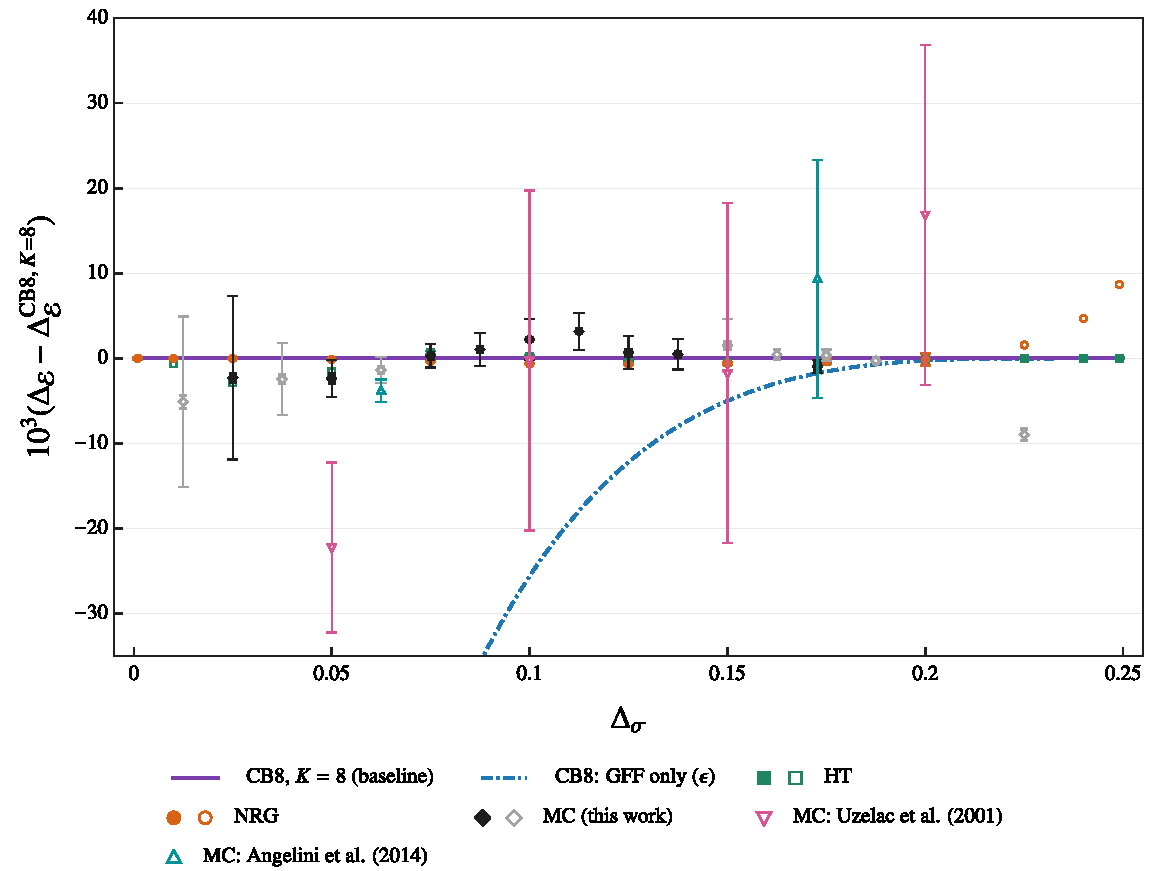
\includegraphics[width=\textwidth]{05_method_dispersion_clean.pdf}
\caption{One dimension: deviations $10^3(\De-\De^{\rm baseline})$ of all displayed reference
points from the $K=8$ baseline, with full error bars, including the published MC values
(rose inverted triangles: Uzelac et al.\ 2001; teal triangles: Angelini et al.\ 2014). Markers as in
Fig.~\ref{fig:methods}. Blue dash-dot: GFF-only CB8, below the frame for $\Ds<0.088$ (it
reaches $-433$ at $\Ds=0$). The $K=5$--$8$ envelope is not drawn; its width is at most
$\sci{4.67}{-3}$, that is $4.67$ in these units.}
\label{fig:dispersion}
\end{figure}

\paragraph{HT and NRG.} At $\Ds=0.15$--$0.2$ the final HT and NRG values agree (differences
at most $\sci{1.0}{-4}$, below the sum of their errors). At $\Ds=0.1$ and $0.125$ the NRG
values lie $\sci{8.7}{-4}$ and $\sci{4.5}{-4}$ below the HT values, $5.8$ and $4.6$ times the
sum of the HT fit half-spread and the NRG error. The gap is of the size of the dependence of
HT on the correction of its truncation artifact: without the correction the truncation
extrapolates $\sci{2.3}{-3}$ and $\sci{6.6}{-4}$ lower at these points ($\sci{1.7}{-3}$ at
$0.075$), and NRG lies between the two limits. The HT note does not combine this dependence
into its error, because the truncation has no strict error bar and an error built after the
gap to NRG had been seen would make the two methods appear to agree \cite{noteHT}. The HT values therefore keep their fit half-spreads, and the difference between
the corrected and uncorrected limits is shown separately.

\paragraph{Do the data select $K=8$ over $K=4$?} The archived $K=4$ and the baseline $K=8$
curves differ by at most $\sci{1.32}{-3}$ (at $\Ds=0.109$). That is less than the width of the
$K=8$ core band at the same points ($\sci{2.0}{-3}$ at $\Ds=0.1$, $\sci{3.0}{-3}$ at $0.125$), so a
preference between them is a choice inside the prescription dependence.
Table~\ref{tab:k4k8} compares the separation with the quoted errors and lists the dependence of
HT on the artifact correction separately.
\begin{itemize}
\item \emph{MC} does not resolve the two curves anywhere: the separation is at most $0.59$
of the sum of $\sigma_{\rm stat}$ and $\sigma_{\rm sys}$ of an accepted value.
\item \emph{HT.} At $\Ds=0.075$ and $0.1$ HT lies above both curves, nearer $K=8$, but its
dependence on the artifact correction ($\sci{1.7}{-3}$, $\sci{2.3}{-3}$) exceeds the separation of the curves
($\sci{1.0}{-3}$, $\sci{1.3}{-3}$), so HT does not decide there. At $0.125$ it lies between the
curves, nearer $K=8$. At $0.15$--$0.2$, where the prescription dependence is small
($\le\sci{1.3}{-4}$), it lies between the curves and nearer $K=4$: $\sci{1}{-5}$ to $\sci{4}{-4}$
above $K=4$ ($2.6$--$12$ errors) and $\sci{9}{-5}$ to $\sci{5}{-4}$ below $K=8$ ($15$--$21$ errors).
\item \emph{NRG} selects $K=8$ only at $\Ds=0.025$, where the separation is $\sci{1.9}{-4}$ and
$K=4$ is $6.2$ errors away. At $0.05$--$0.15$ it lies between the curves, more than $2.5$
errors from each: nearer $K=8$ at $0.05$, $0.075$ and, marginally, $0.1$ ($19.1$ against
$19.7$ errors), nearer $K=4$ at $0.125$ and $0.15$. At $0.175$, $0.2$ and $\Ds\le0.01$ the separation is below two errors.
\end{itemize}
So the precise data resolve the $K=4$--$K=8$ difference at several points, but no method
favors $K=8$ over its range. Where both curves are resolved, HT and NRG mostly lie between
them, and at $0.15$--$0.2$, where HT is most precise and depends least on the artifact
correction, they lie nearer $K=4$. An earlier version of this note justified $K=8$ by its
agreement with HT and NRG. That argument relied on the HT fit half-spread alone at
$\Ds=0.1$--$0.125$ and on earlier NRG values; it does not survive the dependence of HT on the
artifact correction, which exceeds the separation at $\Ds=0.075$ and $0.1$, and it is
withdrawn. The choice $K=8$ rests only on its a priori motivation: these are all the
short-range coefficients we have, and at fixed $K$ the prescriptions then spread much less
than with $K=4$ (core band at $\Ds=0.05$: $\sci{2.3}{-4}$ against $\sci{3.4}{-3}$) and depend
less on $\bL$ (Secs.~\ref{sec:res1d} and~\ref{sec:robust}). It was fixed after the comparison
data had been seen, and taken together these data do not favor it over $K=4$.

\begin{table}[htbp]\centering\scriptsize\setlength{\tabcolsep}{2.5pt}
\begin{tabular}{@{}r r r r r r l r r r l@{}}
\toprule
 & & \multicolumn{5}{c}{HT (corrected)} & \multicolumn{4}{c}{NRG}\\
\cmidrule(lr){3-7}\cmidrule(l){8-11}
$\Ds$ & $10^4(F_4{-}F_8)$ & $10^4(y{-}F_8)$ & err & $z_8$, $z_4$ & corr.$-$unc. & & $10^4(y{-}F_8)$ & err & $z_8$, $z_4$ & \\ \midrule
0.025 & $-1.89$ & $\cdot$ & $\cdot$ & $\cdot$ & $\cdot$ &  & $-0.10$ & $\sci{2.9}{-5}$ & $-0.4$, $+6.2$ & near 8\\
0.05 & $-6.12$ & $\cdot$ & $\cdot$ & $\cdot$ & $\cdot$ &  & $-1.19$ & $\sci{2.7}{-5}$ & $-4.5$, $+18.4$ & b(8)\\
0.075 & $-10.43$ & $+6.99$ & $\sci{2.0}{-4}$ & $+3.5$, $+8.8$ & $\sci{1.7}{-3}$ & o(8)$^\dagger$ & $-3.67$ & $\sci{3.0}{-5}$ & $-12.3$, $+22.7$ & b(8)\\
0.1 & $-12.99$ & $+2.31$ & $\sci{1.2}{-4}$ & $+2.0$, $+13.2$ & $\sci{2.3}{-3}$ & o(8)$^\dagger$ & $-6.39$ & $\sci{3.3}{-5}$ & $-19.1$, $+19.7$ & b(8)\\
0.125 & $-12.48$ & $-3.09$ & $\sci{4.3}{-5}$ & $-7.2$, $+21.8$ & $\sci{6.6}{-4}$ & b(8) & $-7.55$ & $\sci{5.4}{-5}$ & $-14.1$, $+9.2$ & b(4)\\
0.15 & $-9.01$ & $-5.03$ & $\sci{3.3}{-5}$ & $-15.4$, $+12.2$ & $\sci{1.3}{-4}$ & b(4) & $-6.06$ & $\sci{1.1}{-4}$ & $-5.3$, $+2.6$ & b(4)\\
0.175 & $-4.37$ & $-3.32$ & $\sci{1.5}{-5}$ & $-21.4$, $+6.8$ & $\sci{3.3}{-5}$ & b(4) & $-3.40$ & $\sci{3.5}{-4}$ & $-1.0$, $+0.3$ & n.r.\\
0.2 & $-1.04$ & $-0.92$ & $\sci{4.7}{-6}$ & $-19.4$, $+2.6$ & $\sci{4.5}{-6}$ & b(4) & $-1.36$ & $\sci{7.1}{-4}$ & $-0.2$, $-0.0$ & n.r.\\
\bottomrule
\end{tabular}
\caption{Can the comparison data tell the $K=4$ and $K=8$ curves apart? $F_K$: CB8 with the
short-range series through $\CSR_K$; $y$: the HT or NRG value; $z_K=(y-F_K)/{\rm err}$. HT err:
half-spread of the accepted fits (quoted); at $\Ds=0.075$ its one-sided allowance $-\sci{5}{-4}$
is not included and would lower $z_8$ to $1.0$. corr.$-$unc.: the HT limit corrected for the
truncation artifact minus the uncorrected limit, shown separately and not combined with err
(Sec.~\ref{sec:cmp1d}). NRG err: chain-depth, kept-state and discretization errors added
linearly. Labels: near 8, within one error of $F_8$ and more than two from $F_4$; b($K$),
between the curves, and o($K$), outside both, more than one error from each and nearer $F_K$;
n.r., separation below two errors. $^\dagger$: the dependence on the artifact correction
exceeds the separation. MC resolves neither curve anywhere. The errors are not
standard deviations; the ratios are descriptive.}
\label{tab:k4k8}
\end{table}

\subsection{Two dimensions}
The finite-cutoff HT values \cite{noteHT} at the largest cutoff ($N=24$ at eleven couplings,
$N=22$ at $\Ds=0.125$ and $0.126$) compare with the curvature baseline as follows
(Fig.~\ref{fig:curves23}, left):
\begin{itemize}
\item At weak coupling, $\Ds\ge0.35$ ($s\le1.3$), HT agrees with CB8 to at most
$\sci{8}{-4}$, inside the core band.
\item In mid-window HT lies above the baseline: $\sci{+2.3}{-3}$ at $\Ds=0.3$,
$\sci{+6.6}{-3}$ at $0.25$, $\sci{+9.9}{-3}$ at $0.2$ and $\sci{+7.3}{-3}$ at $0.175$.
At $s=1.4$--$1.5$ ($\Ds=0.3$--$0.25$) HT lies within the spread of the endpoint
constructions, inside the core band of the tangent construction. At $s=1.6$--$1.65$
($\Ds=0.2$--$0.175$) HT is above every construction, by about $\sci{3}{-3}$ above the upper
edge of the tangent core band. The cutoff dependence does not show whether this excess
survives at infinite cutoff. At $s=1.4$ and $1.5$ HT rises monotonically with $N$, so if the
rise continues the $N=24$ values are lower bounds. At $s=1.6$, however, it is flat from $N=18$
on and falls by $\sci{5}{-5}$ in the last step, and at $s=1.65$ it falls steadily from $N=10$
on (by $\sci{5.3}{-3}$ up to $N=24$, $\sci{1.0}{-3}$ in the last step), so larger cutoffs could
reduce the excess there.
\item Near the short-range end ($\Ds\le0.15$) HT drifts downward, away from the exact
endpoint value $1$ ($0.940$ at $\Ds=\frac18$, $N=22$), and is not usable.
\end{itemize}
The discrepancy is not assigned to either method: the cutoff dependence and the artifact
correction of HT, the uncomputed orders and the endpoint assumptions all remain. The
thirteen published MC values have quoted errors from $0.006$ to $0.034$ (and $0.10$ for
Angelini et al.\ at $s=\frac74$). Away from $s=\frac74$ they lie within two quoted errors of
both CB8 and HT, so they cannot separate them; at $s=\frac74$ they agree with the exact value
$1$, which HT misses. Luijten's two estimators on the same data differ by up to $0.05$. The
project's own 2d MC values are conditional or model-limited \cite{noteMC}, so only
finite-size exponents are available (Table~\ref{tab:mc2d}). The exponents
$\Delta_{\rm eff}(U_4)$ of the largest lattice pair ($L=512\to1024$) agree with the curvature
baseline to $\sci{1.5}{-3}$ at $s=1.2$--$1.4$. There the endpoint constructions differ from it
by up to $\sci{4.7}{-3}$, so the exponents do not select one. Toward both ends ($s=1.05$,
$1.1$ and $1.5$--$1.7$) they fall short of the baseline by $0.005$ to $0.02$.

\begin{table}[htbp]\centering\small
\begin{tabular}{@{}r r l r r r r@{}}
\toprule
$s$ & $\Ds$ & label & $\Delta_{\rm eff}(U_4)$ & curvature CB8 & $10^3$(MC$-$CB8) & $10^3\,\max|{\rm constr.}-{\rm CB8}|$\\ \midrule
1.05 & 0.475 & conditional & 0.9702(25) & 0.985836 & $-15.65$ & 0.00\\
1.1 & 0.45 & conditional & 0.9659(23) & 0.975429 & $-9.51$ & 0.02\\
1.2 & 0.4 & conditional & 0.9631(22) & 0.962567 & $+0.56$ & 0.54\\
1.3 & 0.35 & model-limited & 0.9584(20) & 0.958099 & $+0.28$ & 2.33\\
1.4 & 0.3 & model-limited & 0.9627(20) & 0.961182 & $+1.54$ & 4.68\\
1.5 & 0.25 & model-limited & 0.9661(18) & 0.971143 & $-5.03$ & 5.69\\
1.6 & 0.2 & model-limited & 0.9698(18) & 0.985419 & $-15.66$ & 7.02\\
1.7 & 0.15 & model-limited & 0.9773(17) & 0.997797 & $-20.49$ & 5.54\\
\bottomrule
\end{tabular}
\caption{Two dimensions: finite-size exponents $\Delta_{\rm eff}(U_4)$ of the project's MC for
the largest lattice pair, $L=512\to1024$, with their statistical errors \cite{noteMC}, against
the curvature baseline. Last column: the largest deviation of the tangent and value
constructions and the GFF-only curve from the baseline. These are not infinite-size values.}
\label{tab:mc2d}
\end{table}

\subsection{Three dimensions}
Against the slope baseline (Fig.~\ref{fig:curves23}, right):
\begin{itemize}
\item HT at $N=20$ is within $\sci{1}{-3}$ of CB8 for $\Ds\ge0.6$ ($s\le1.8$), for example
$\sci{-2.2}{-4}$ at $\Ds=0.7$ and $\sci{-9.3}{-4}$ at $\Ds=0.65$. Toward the short-range end
it lies above, by $\sci{1.2}{-3}$ at $\Ds=0.575$ rising to $\sci{6.6}{-3}$ at $\Ds=S$, where HT
gives $1.41924$ against the exact $E=1.41262528$; as in $d=2$, HT fails near the short-range
end, here lying above the curve rather than below it.
\item The project's MC value at $s=1.6$ \cite{noteMC}, $\De=1.47314\pm0.00118\,({\rm
stat})\pm0.00230\,({\rm sys})$, lies $\sci{1.0}{-3}$ above CB8 ($1.47214$). It is accepted
only under amendment P1 (Table~\ref{tab:refstatus}), adopted after the protocol had been
applied to the production data; $\sigma_{\rm sys}$ is the half-range of the values over the
admissible extrapolation series.
\item The project's extrapolations that are not accepted, at $s=1.7$, $1.85$ and $1.9$
(cross-check failed or unavailable), lie $0.022$ to $0.033$ above CB8.
\item Luijten's thesis gives $1.477(16)$ at $s=1.6$ and $1.46(4)$ at $s=1.8$, $+0.3$ and
$+0.6$ quoted errors from CB8; Luijten calls these results rather poor (lattices up to
$L=64$, correction exponent fixed by hand).
\item Bootstrap kinks read off Fig.~11 of Ref.~\cite{Behan:2023ile} (conjectured
identification) give $1.470$, $1.450$, $1.432$, $1.415$ at $s=1.593$, $1.685$, $1.778$,
$1.871$ (read-off error about $\pm0.005$), below CB8 by $0.004$, $0.004$, $0.007$, $0.010$. The
gap grows toward the short-range end, where CB8 imposes $c_1=0.273$; the kink at $s=1.871$
implies a smaller slope. A functional-RG truncation \cite{Defenu:2014bea} departs by up to
$0.03$ near the short-range end, where its thermal exponent, about $1.543$ as read off its
Fig.~2, stays below the 3d Ising value $1.5874$.
\end{itemize}

%====================================================================
\section{Robustness}\label{sec:robust}
%====================================================================
\subsection{Held-out coefficients}
A finite-order test that uses no comparison data is to withhold the last known
coefficient, construct the approximant from the lower ones and re-expand it to predict
the withheld one. This tests finite-order predictive power, not asymptotic dominance.
Tables~\ref{tab:heldout1} and~\ref{tab:heldout23} collect the results;
Fig.~\ref{fig:instanton} shows the one-dimensional ones together with the matched
CB$-$PB differences.

\begin{figure}[htbp]\centering
\widefig{02_instanton_clean.pdf}
\caption{One dimension: conformal Borel against Pad\'e--Borel. Top: matched differences
$10^3(\De^{\rm CB8}-\De^{{\rm PB}[5/3]})$ with the same coefficients, endpoint input
$F^{\rm SR}_K$, order, variable and $\bL=3$; left in $v$ for $K=4$ (archived), $5$, $6$, $7$; right in
$\epsilon$ for $K=4,6,7$ (where PB$[5/3]$ is admissible). Bottom: absolute relative errors of
held-out $C_6,C_7,C_8$ predicted from the preceding coefficients; left for the GFF-only
series (independent of $K$), right for the endpoint-$v$ construction with $K=8$ (dark) and
$K=4$ (light). PB shapes as selected by the rule of Sec.~\ref{sec:pade} ($K=8$: $[4/1]$, $[4/2]$, $[3/4]$;
$K=4$ and GFF-only: $[3/2]$, $[4/2]$, $[5/2]$). The $C_8$ bars use the final $C_8(1)$
(allowance about $0.21\%$).}
\label{fig:instanton}
\end{figure}

\begin{table}[htbp]\centering\small
\begin{tabular}{@{}l r r r@{}}
\toprule
Construction ($\bL=3$) & $C_6$ & $C_7$ & $C_8$\\ \midrule
GFF only, CB & 11.03 & 1.58 & 1.55\\
GFF only, PB ($[3/2],[4/2],[5/2]$) & 5.70 & 0.44 & 0.33\\
Endpoint-$v$, $K=8$, CB & 10.95 & 5.93 & 0.94\\
Endpoint-$v$, $K=8$, PB ($[4/1],[4/2],[3/4]$) & 3.86 & 0.17 & 0.50\\
Endpoint-$v$, $K=4$, CB & 7.23 & 0.37 & 0.81\\
Endpoint-$v$, $K=4$, PB ($[3/2],[4/2],[5/2]$) & 2.53 & 0.16 & 0.44\\
\bottomrule
\end{tabular}
\caption{One dimension: absolute relative errors (\%) of held-out coefficients. The
targets $C_6,C_7$ are unchanged; for $C_8$ the final value is the target, and the
predictions themselves do not depend on it.}
\label{tab:heldout1}
\end{table}

\begin{table}[htbp]\centering\small
\begin{tabular}{@{}c rrrr c rrrr@{}}
\toprule
& \multicolumn{4}{c}{$d=2$} && \multicolumn{4}{c}{$d=3$}\\
\cmidrule{2-5}\cmidrule{7-10}
& \multicolumn{2}{c}{GFF only} & \multicolumn{2}{c}{with SR input} && \multicolumn{2}{c}{GFF only} & \multicolumn{2}{c}{with SR input}\\
Target & CB & PB & CB & PB && CB & PB & CB & PB\\ \midrule
$C_5$ & 7.75 & 37.99 & 44.88 & 2.26 && 1.67 & 1.56 & 9.72 & 7.00\\
$C_6$ & 9.25 & 5.16 & 22.31 & 4.57 && 4.32 & 2.42 & 0.80 & 18.25\\
$C_7$ & 0.81 & 0.18 & 5.82 & 6.93 && 1.64 & 1.16 & 1.99 & 0.10\\
$C_8$ & 1.24 & 0.22 & 2.99 & 0.31 && 0.37 & 0.52 & 0.33 & 0.16\\
\bottomrule
\end{tabular}
\caption{Two and three dimensions: absolute relative errors (\%) of held-out coefficients
at the baseline $\bL$. GFF only: the series resummed directly; with SR input: the curvature
($d=2$) and slope ($d=3$) constructions. PB shapes as selected by the rule of
Sec.~\ref{sec:pade}.}
\label{tab:heldout23}
\end{table}

Different orders, dimensions and constructions favor different families. For the
newly measured $C_8$, the GFF-only PB prediction is closer in $d=1$ and $d=2$, CB is
closer in $d=3$. In $d=1$ the $K=8$ CB prediction of $C_8$ is $0.94\%$ off, which is $4.4$
times the allowance of $C_8(1)$ ($0.21\%$). An accurate PB prediction of $C_8$ also does not
guarantee an admissible eighth-order PB curve of the matched shape once $C_8$ is supplied: at
$K=8$ in $d=1$ only $[3/5]$ survives at eighth order, and in $d=3$ no eighth-order candidate
survives at $\bL=4$. These tests support keeping both families and the
explicit admissibility diagnostics. They do not validate an instanton amplitude or establish
an advantage of supplying the action.

\subsection{Order and Borel--Leroy stability}
Figure~\ref{fig:stability} shows the order and $\bL$ dependence in $d=1$. At $K=8$ the CB
curves at orders 6 and 7 differ from CB8 by at most $\sci{8.8}{-4}$ and $\sci{2.2}{-4}$; changing
$\bL$ to $2$ or $4$ moves the curve by at most $\sci{1.4}{-4}$, while $\bL=0$ moves it by up to
$\sci{2.9}{-3}$ (at $K=4$: $\sci{1.8}{-2}$). The short-range input thus also stabilizes the
Borel--Leroy dependence. Varying $1/\Ae$ by $\pm20\%$ moves the $K=8$ baseline by at most
$\sci{1.0}{-3}$ (scale $0.8$), and by at most $\sci{1.6}{-4}$ for the other variations. In
$d=2$ and $3$, adding $C_8$ changed the curves by at most $\sci{8.3}{-4}$ and $\sci{1.1}{-5}$
(Sec.~\ref{sec:res23}). Small order-to-order changes are stability observations, not an
estimate of the total error.

\begin{figure}[htbp]\centering
\widefig{03_stability_clean.pdf}
\caption{One dimension: finite-order stability. Top row: $K=8$ baseline; bottom row: the
archived $K=4$ construction (with the final $C_8(1)$). Left: deviations
$10^3(\De-\De^{\rm CB8})$ of CB at orders 6, 7 and of the PB controls $[4/2]$, $[5/2]$, $[5/3]$
($\bL=3$, drawn only where admissible; at $K=8$ and order 8 no PB is drawn). Right: deviations of
CB8 at $\bL=0,2,4$ from $\bL=3$. Vertical ranges differ between the right panels.}
\label{fig:stability}
\end{figure}

\subsection{\texorpdfstring{Coefficient precision, the final $C_8(1)$ and a ninth coefficient}{Coefficient precision, the final C8(1) and a ninth coefficient}}
For fixed CB parameters the reconstruction is affine in the input coefficients, so
coefficient sensitivity can be computed exactly from unit responses $J_n=\partial F/\partial
C_n$. We report $U=\sum_{n=6}^8|J_n|\,\delta C_n$, the sum of absolute responses to the
allowances. This would be a worst-case bound only if the allowances were rigorous
simultaneous bounds, which they are not; with a covariance matrix $\Sigma$ the variance would
be $J^{\mathsf T}\Sigma J$. Four sources of uncertainty must be kept separate: numerical
integration (negligible), input coefficients ($U$), prescription and endpoint construction (the
bands), and the theoretical assumptions about the endpoint and the instanton.

\begin{figure}[htbp]\centering
\widefig{04_precision_clean.pdf}
\caption{One dimension: coefficient precision. Top row $K=8$, bottom row $K=4$ (archived
construction, current inputs). Left: $10^4\,U$ for the current allowances
($\delta C_8=17000$, $\delta C_7=41$, $\delta C_6=\sci{4.9}{-7}$), for $\delta C_8/10$, and with $C_8$
exact. Right: $10^3\,\delta\De$ for a hypothetical $C_9$: the shift if
$C_9=C_9^{\rm hyp}$ and the responses to $1\%$ and $5\%$ of $|C_9^{\rm hyp}|$. Top:
$C_9^{\rm hyp}=\sci{-2.178401719}{8}$, the CB prediction of the $K=8$ baseline, so its shift
vanishes identically. Bottom: $C_9^{\rm hyp}=\sci{-2.190506633}{8}$, the archived $K=4$
PB$[5/3]$ prediction made with the previous $C_8(1)$, kept as a fixed scenario value. These are
sensitivity scenarios, not confidence intervals; $C_9$ has not been calculated.}
\label{fig:precision}
\end{figure}

At $\Ds=0.1$ and $K=8$, $U=\sci{3.76}{-5}$ with the final allowance; dividing $\delta C_8$ by ten
gives $\sci{9.69}{-6}$, and the floor with $C_8$ exact (set by $\delta C_7$) is $\sci{6.59}{-6}$.
The corresponding values at $K=4$ are $\sci{2.34}{-4}$, $\sci{5.96}{-5}$ and $\sci{4.03}{-5}$. A
tenfold better $C_8$ would thus improve the input budget by a factor $3.9$ but leave the
prescription envelope, about a hundred times larger, unchanged.

\paragraph{What the final $C_8(1)$ changed.} Replacing $8066723.343\pm33000$ by
$8059766.723\pm17000$ (a shift of $-6957$) moves the $K=8$ baseline down by at most
$\sci{2.0}{-5}$ (at $\Ds=0.141$; $\sci{-1.27}{-5}$ at $\Ds=0.1$). It lowers the upper edge of
the envelope by up to $\sci{1.9}{-4}$: the width at $\Ds=0.1$ goes from $\sci{3.84}{-3}$ to
$\sci{3.64}{-3}$, and the maximum width $\sci{4.67}{-3}$ is unchanged. It roughly halves the
$C_8$ term of $U$ ($\sci{6.02}{-5}\to\sci{3.10}{-5}$ at $\Ds=0.1$, so that $U$ falls from
$\sci{6.68}{-5}$ to $\sci{3.76}{-5}$), and it changes the mismatch ratio at $n=8$ from $0.1578$
to $0.1576$. With the previous value every program reproduces the archived outputs to
$\sci{8.4}{-15}$.

\paragraph{A ninth coefficient.} $C_9$ has not been computed. At fixed CB parameters the
ninth-order curve obeys the exact identity
\begin{equation}
 F_9(x)-F_8(x)=J_9(x)\,\bigl[C_9-C_9^{\rm CB8}\bigr],\qquad J_9=\frac{\partial F_9}{\partial C_9},
 \label{eq:C9}
\end{equation}
where $C_9^{\rm CB8}$ is the coefficient implied by the eighth-order approximant; supplying
that value adds no information. The $K=8$ baseline implies
$C_9^{\rm CB8}=\sci{-2.178401719}{8}$; the only admissible eighth-order PB at $K=8$, $[3/5]$,
predicts $\sci{-2.181155}{8}$, and the $K=4$ CB8 implies $\sci{-2.19002}{8}$. These are correlated
predictions, not a calculation. At $\Ds=0.1$ a change of $1\%$ of $|C_9|$ would move the
$K=8$ curve by $\sci{3.5}{-4}$ (at $K=4$: $\sci{2.2}{-3}$). Adding the ninth order also amplifies
the inherited sensitivity to $C_8$: at $\Ds=0.1$ the $C_8$ term of $U$ grows from $\sci{3.1}{-5}$
to $\sci{2.9}{-4}$ at $K=8$ (from $\sci{1.9}{-4}$ to $\sci{1.8}{-3}$ at $K=4$). Simply appending
$C_9$ is therefore not guaranteed to improve the curve: a useful ninth order needs an
independently computed $C_9$, sufficient precision on $C_8$, and renewed prescription checks.

%====================================================================
\section{Limitations and open problems}\label{sec:open}
%====================================================================
\begin{enumerate}
\item \textbf{Reporting prescription.} The number $K=8$ of imposed short-range
coefficients, and the range $K=5$--$8$ of the envelope, were fixed after the comparison data
had been seen. $K=8$ is motivated a priori only (all short-range coefficients); choosing the
narrowest core band would give $K=7$. Whether the endpoint variable ($v$ or $\epsilon$) belongs in the
envelope is open.
\item \textbf{Endpoint assumptions.} The constructions assume that the resummed remainder is
regular at the short-range end. Logarithms beyond the imposed terms are not excluded. The
two-dimensional $c_2$ carries a formal analytic-MS qualification, the three-dimensional
$c_1$ a conditional spectral range; the one-dimensional $\CSR_n$ beyond the published orders
are project results with their own assumptions, and the short form of $\CSR_8$ is unproved.
In $d=2$ the endpoint construction is the largest uncertainty in mid-window.
\item \textbf{The amplitude.} The cancellation of the regulator dependence of the bubble
action in the one-loop amplitude (Sec.~\ref{sec:amplitude}) should be derived explicitly. The
derivation must keep the integration limits, determinant, measure, legs and counterterms
through the simple-pole residue, for the size coordinate and for its rescaled form.
\item \textbf{Next order and approach to large order.} The coefficient $d_1$ needs the
two-loop fluctuations, the subleading size integral and the direct mass insertion, and
possibly logarithms. Its known part already gives $-30\%$ at $n=8$; further corrections may
be needed before eighth order can test $K_I$.
\item \textbf{Dominance.} The Sobolev bound identifies the least-action real saddle; it does
not settle complex saddles, integration cycles, multi-instanton sectors, non-instanton
factorial mechanisms or the uniformity of the renormalized expansion.
\item \textbf{Two and three dimensions.} Only the actions and the power counting are
available. A renormalized determinant and amplitude would be needed for amplitude-based
tests.
\item \textbf{Coefficients.} A covariance model for $C_6,C_7,C_8$ is missing. A ninth
coefficient would be a useful test of the predictions only with adequate precision on $C_8$
(Sec.~\ref{sec:robust}).
\item \textbf{Comparisons.} In $d=1$ the final HT and NRG values differ at $\Ds=0.1$ and
$0.125$ by $5.8$ and $4.6$ times the sum of their quoted errors. The gap is of the size of the
dependence of HT on the artifact correction, which the HT error does not include
(Sec.~\ref{sec:cmp1d}), and its origin is open. HT and NRG resolve the $K=4$--$K=8$ difference at
several points but lie between the two curves there (Table~\ref{tab:k4k8}), so they cannot
justify the choice of $K$. In $d=2$ and $3$ HT is available only at finite cutoff; the $d=2$
mid-window excess of HT over every endpoint construction (about $\sci{3}{-3}$ beyond their
core bands at $s=1.6$--$1.65$) is unresolved, and the cutoff dependence there does not show
that it survives at infinite cutoff. Published MC is too imprecise to discriminate, and in
$d=3$ there is a single accepted project MC point. Continuum HT extrapolations and MC with
controlled systematics would be the most informative additions.
\item \textbf{Interpretation of the $d=1$ endpoint.} The fixed-point-merger reading of the
square-root branch point, and the radius $\simeq\frac12$ suggested by the short-range series,
should be checked against more coefficients or an independent argument.
\end{enumerate}

%====================================================================
\appendix
\section{Formulas and parameters}\label{app:formulas}
%====================================================================
\paragraph{Conformal Borel coefficients.} For the resummed series $f(z)=\sum_{j\le m}f_jz^j$
with action $A$,
\begin{equation}
 p_k=\sum_{j=0}^k\frac{f_j\,(4A)^j}{\Gamma(j+\bL+1)}\,(-1)^{k-j}\binom{\alpha-2j}{k-j},\qquad
 \cR_m^{\rm CB}[f](z)=\int_0^\infty e^{-u}u^{\bL}\,
 \frac{\sum_{k=0}^mp_k\,w(zu)^k}{[1-w(zu)]^\alpha}\dd u ,
 \label{eq:pk}
\end{equation}
which reproduces the Taylor polynomial through order $m$; for integer $\alpha-2j$ the
generalized binomial coefficient is the polynomial one. The inverse map
$w(t)=\sum_{k\ge1}(-1)^{k-1}\frac{1}{k+1}\binom{2k}{k}(t/4A)^k$ gives an independent
round-trip check.

\paragraph{Pad\'e--Borel.} With $d_k=f_k/\Gamma(k+\bL+1)$, the denominator of $[L/M]$ solves
$\sum_{j=1}^Mq_jd_{k-j}=-d_k$ for $k=L+1,\dots,m$, and $p_k=\sum_{j=0}^{\min(k,M)}q_jd_{k-j}$
with $q_0=1$. The Pad\'e denominator depends nonlinearly on the coefficients, so PB curves are
not affine in the inputs.

\paragraph{Series operations and quadrature.} Products, powers $(1-z)^p$ and compositions are
formed with truncation after each operation, in 65-digit arithmetic. The Laplace integral uses
240-point generalized Gauss--Laguerre quadrature for weight $u^{\bL}e^{-u}$ (Jacobi matrix with
diagonal $2k+\bL+1$ and off-diagonal $\sqrt{k(k+\bL)}$), checked against 120 nodes, adaptive
integration and selected 65-digit integrals. For the one-dimensional CB curves the 240-node and
adaptive results agree to $\sci{1.1}{-15}$, the 65-digit checks to $\sci{5.2}{-16}$, and the
displayed PB curves to $\sci{4.0}{-15}$. Formal re-expansion reproduces the input coefficients.
These checks validate the evaluation of each approximant, not its distance from the exact theory.

\paragraph{Grids.} The one-dimensional dense grid has 1004 points (1001 equally spaced on
$[0,\frac14]$ plus the special comparison abscissae); the matched CB/PB comparison uses 502
points. The two- and three-dimensional curves have 754 and 763 stored samples.

\paragraph{Scan parameters.} Table~\ref{tab:params} collects all prescription parameters.

\begin{table}[htbp]\centering\small\setlength{\tabcolsep}{3.5pt}
\begin{tabular}{@{}l l l l@{}}
\toprule
 & $d=1$ & $d=2$ & $d=3$\\ \midrule
Resummed variable & $v=1-2\sqrt{\Ds}$ & $\epsilon$ & $\epsilon$\\
CB action & $A_v=\Ae/2=0.25703245$ & $\Ae=9/8$ & $\Ae=1.92343326$\\
Endpoint input & $\CSR_1,\dots,\CSR_8$ ($K=8$) & $1$, $0$, $c_2$ & $E$, $c_1$\\
Endpoint controls & $K=4$--$7$, endpoint-$\epsilon$ & tangent, value & value\\
Without SR input & GFF-only & GFF-only & GFF-only\\
Orders & $6,7,8$ & $6,7,8$ & $6,7,8$\\
Core $\bL$ & $2,3,4$ & $2.5,3.5,4.5$ & $3,4,5$\\
Wide $\bL$ & $0,1,\dots,6$ & $0,1.5,2.5,\dots,6.5$ & $0,2,3,\dots,7$\\
$\alpha$ (core; wide) & $-1,0,1$; $-2,\dots,2$ & $-1,0,1$; $-2,\dots,2$ & $-1,0,1$; $-2,\dots,2$\\
Action variations & $1/A\times0.8,0.9,1.1,1.2$ & same & same\\
PB control & $[5/3]$ ($K\le7$) & PB8 $[5/3]$ & PB7 $[3/4]$; PB8 $[5/3]$ at $\bL=0$\\
Stored grid & 1004 points & 754 points & 763 points\\
\bottomrule
\end{tabular}
\caption{Resummation parameters. The baseline uses order 8, the middle core $\bL$ and
$\alpha=0$; the PB controls use the baseline $\bL$ unless stated.}
\label{tab:params}
\end{table}

\paragraph{One-dimensional comparison data.} Table~\ref{tab:refs1d} lists every
one-dimensional value compared in this note, with its residual from the baseline.

{\small
\begin{longtable}{@{}l r r r r l r@{}}
\caption{One-dimensional comparison data \cite{noteHT,noteNRG,noteMC,Uzelac:2001lc,Angelini:2014koy},
labels as in Table~\ref{tab:refstatus}. ``err'': for HT the half-spread of the accepted fits,
for NRG the chain-depth, kept-state and discretization errors added linearly, for MC
$\sigma_{\rm sys}$, for published MC the quoted error; ``stat'': the MC statistical error. A dot
means none supplied. MC $\Delta_{\rm eff}$: finite-size exponents of the largest lattice pair
(sizes in parentheses), not infinite-size values. The last column is
$10^3(\De-\De^{\rm baseline})$.}\label{tab:refs1d}\\
\toprule Method & $\Ds$ & $\De$ & err & stat & status & resid.\\ \midrule\endfirsthead
\toprule Method & $\Ds$ & $\De$ & err & stat & status & resid.\\ \midrule\endhead
\midrule\multicolumn{7}{r}{continued on the next page}\\\endfoot
\bottomrule\endlastfoot
HT & 0.249 & 0.4993436 & $\sci{9.3}{-8}$ & $\cdot$ & final & $-0.00$\\
HT & 0.24 & 0.4942198 & $\sci{2.6}{-6}$ & $\cdot$ & final & $+0.00$\\
HT & 0.225 & 0.4880804 & $\sci{5.2}{-6}$ & $\cdot$ & final & $-0.00$\\
HT & 0.2 & 0.4830244 & $\sci{4.7}{-6}$ & $\cdot$ & final & $-0.09$\\
HT & 0.175 & 0.4839086 & $\sci{1.5}{-5}$ & $\cdot$ & final & $-0.33$\\
HT & 0.15 & 0.4912086 & $\sci{3.3}{-5}$ & $\cdot$ & final & $-0.50$\\
HT & 0.125 & 0.5061186 & $\sci{4.3}{-5}$ & $\cdot$ & final & $-0.31$\\
HT & 0.1 & 0.5304771 & $\sci{1.2}{-4}$ & $\cdot$ & final & $+0.23$\\
HT & 0.075 & 0.5673260 & $\sci{2.0}{-4}$ & $\cdot$ & one-sided & $+0.70$\\
HT & 0.05 & 0.6206712 & $\cdot$ & $\cdot$ & unstable ($N=40$) & $-1.56$\\
HT & 0.025 & 0.7105771 & $\cdot$ & $\cdot$ & no limit ($N=40$) & $-2.86$\\
HT & 0.01 & 0.8091106 & $\cdot$ & $\cdot$ & no limit ($N=40$) & $-0.64$\\
HT & 0.001 & 0.9693379 & $\cdot$ & $\cdot$ & no limit (not shown) & $+31.91$\\
NRG & 0.249 & 0.508030 & $\cdot$ & $\cdot$ & not converged & $+8.69$\\
NRG & 0.24 & 0.498922 & $\cdot$ & $\cdot$ & not converged & $+4.70$\\
NRG & 0.225 & 0.489668 & $\cdot$ & $\cdot$ & not converged & $+1.58$\\
NRG & 0.2 & 0.482980 & $\sci{7.1}{-4}$ & $\cdot$ & final & $-0.14$\\
NRG & 0.175 & 0.483900 & $\sci{3.5}{-4}$ & $\cdot$ & final & $-0.34$\\
NRG & 0.15 & 0.491106 & $\sci{1.1}{-4}$ & $\cdot$ & final & $-0.61$\\
NRG & 0.125 & 0.505672 & $\sci{5.4}{-5}$ & $\cdot$ & final & $-0.76$\\
NRG & 0.1 & 0.529608 & $\sci{3.3}{-5}$ & $\cdot$ & final & $-0.64$\\
NRG & 0.075 & 0.566260 & $\sci{3.0}{-5}$ & $\cdot$ & final & $-0.37$\\
NRG & 0.05 & 0.622115 & $\sci{2.7}{-5}$ & $\cdot$ & final & $-0.12$\\
NRG & 0.025 & 0.713422 & $\sci{2.9}{-5}$ & $\cdot$ & final & $-0.01$\\
NRG & 0.01 & 0.809747 & $\sci{4.7}{-5}$ & $\cdot$ & final & $-0.00$\\
NRG & 0.001 & 0.937424 & $\sci{1.1}{-4}$ & $\cdot$ & final & $-0.00$\\
MC & 0.0125 & 0.78404 & 0.01003 & 0.00077 & cross-check unavailable & $-5.11$\\
MC & 0.025 & 0.71115 & 0.00959 & 0.00049 & accepted ($\sigma_{\rm sys}$-dominated) & $-2.28$\\
MC & 0.0375 & 0.65904 & 0.00425 & 0.00051 & cross-check unavailable & $-2.42$\\
MC & 0.05 & 0.61987 & 0.00220 & 0.00055 & accepted & $-2.36$\\
MC & 0.0625 & 0.59003 & 0.00150 & 0.00035 & cross-check unavailable & $-1.36$\\
MC & 0.075 & 0.56694 & 0.00139 & 0.00037 & accepted & $+0.31$\\
MC & 0.0875 & 0.54761 & 0.00194 & 0.00032 & accepted & $+1.05$\\
MC & 0.1 & 0.53248 & 0.00242 & 0.00020 & accepted ($\sigma_{\rm sys}$-dominated) & $+2.23$\\
MC & 0.1125 & 0.52020 & 0.00217 & 0.00025 & accepted ($\sigma_{\rm sys}$-dominated) & $+3.17$\\
MC & 0.125 & 0.50710 & 0.00193 & 0.00035 & accepted & $+0.67$\\
MC & 0.1375 & 0.49856 & 0.00180 & 0.00030 & accepted ($\sigma_{\rm sys}$-dominated) & $+0.48$\\
MC & 0.15 & 0.49325 & 0.00306 & 0.00041 & cross-check failed & $+1.54$\\
MC & 0.1625 & 0.48761 & $\cdot$ & 0.00058 & conditional & $+0.47$\\
MC & 0.1727335 & 0.48368 & 0.00078 & 0.00052 & accepted & $-0.97$\\
MC & 0.175 & 0.48460 & 0.00067 & 0.00035 & cross-check failed & $+0.36$\\
MC & 0.1875 & 0.48263 & $\cdot$ & 0.00030 & conditional & $-0.28$\\
MC & 0.225 & 0.47912 & $\cdot$ & 0.00068 & conditional & $-8.96$\\
MC $\Delta_{\rm eff}$ & 0.2125 & 0.4784 & $\cdot$ & 0.0015 & model-limited ($256$k$\to512$k) & $-6.43$\\
MC $\Delta_{\rm eff}$ & 0.2375 & 0.4826 & $\cdot$ & 0.0015 & model-limited ($128$k$\to256$k) & $-10.41$\\
Uzelac 2001 & 0.05 & 0.600 & 0.010 & $\cdot$ & published & $-22.23$\\
Angelini 2014 & 0.0625 & 0.5876 & 0.0013 & $\cdot$ & published & $-3.79$\\
Uzelac 2001 & 0.1 & 0.53 & 0.02 & $\cdot$ & published & $-0.25$\\
Uzelac 2001 & 0.15 & 0.49 & 0.02 & $\cdot$ & published & $-1.71$\\
Angelini 2014 & 0.1727335 & 0.494 & 0.014 & $\cdot$ & published & $+9.35$\\
Uzelac 2001 & 0.2 & 0.50 & 0.02 & $\cdot$ & published & $+16.88$\\
\end{longtable}}

%====================================================================
\section{Reproduction}\label{app:repro}
%====================================================================
Everything in this note is reproduced from the folder \file{Resummation/} of the public
repository. Paths below are relative to it. The programs regenerate the resummations, the
sensitivity analyses and the comparisons from the coefficients and the comparison data; they do
not regenerate graph integrals, HT spectra, NRG runs or MC samples, which come from the sibling
folders \file{GFF/}, \file{HT/}, \file{NRG/} and \file{MC/} (frozen copies in
\file{data/inputs/}, listed with their sources in \file{data/inputs/INPUTS.json}).

\paragraph{Packages.} \file{code/resum_d1/}: the one-dimensional resummation of
Secs.~\ref{sec:methods}--\ref{sec:robust} (endpoint construction with the short-range series
through $\CSR_K$, the $C_8(1)$ switch, curves, envelopes, matched CB/PB comparisons, held-out
tests, $C_9$ scenarios, allowance budgets, reference residuals, the instanton-mismatch table and
the $K=4$/$K=8$ table). \file{code/resum_d23/}: the two- and three-dimensional resummations,
the GFF-only CB3 curves and the table of published MC values. \file{code/instanton/}: the
critical bubble, the amplitude $K_I$ and its benchmarks (Sec.~\ref{sec:largeorder}).
\file{code/comparison/}: the comparison numbers of Sec.~\ref{sec:compare}. The production files
ship unchanged with their production layout and a dated sha256 list
(\file{public/SNAPSHOT.sha256}); the tools added for the public replay are in each package's
\file{public/} and \file{public.mk}.

\paragraph{Commands.} From \file{Resummation/}:
\begin{verbatim}
make test           # fast tests of every package (1 min)
make replay         # every quoted number, shipped records (1 min)
make replay-full    # rerun the resummations, compare outputs (3 min)
make check-inputs   # frozen inputs against the sibling folders
\end{verbatim}
\texttt{make replay} recomputes every number of the sections on resummation and on the
comparison of the paper \cite{LRIpaper} and of its paragraph on higher orders, and the
entries of its results tables that come from this folder: the resummed values in $d=1,2,3$, the
HT values at the largest cutoff in $d=2,3$ and the MC Binder exponents in $d=2$
(\file{results/quoted_numbers.json}). It compares each value, rounded half-up to the printed
digits, with the printed text (the MC exponents with their errors by the PDG rule). The map from each number to its record, command
and tolerance is in \file{results_map.md} (per package in
\file{code/<package>/public/results_map.md}). It also regenerates, byte for
byte, the tables derived from the frozen inputs (the table of one-dimensional comparison data,
the $K=4$/$K=8$ table of Sec.~\ref{sec:compare}, the published-MC table and the comparison tables
in \file{results/comparison/}), and checks the data behind the two figures of the paper
(\file{results/figures/*.csv}). \texttt{make replay-full} reruns the one-dimensional chain
(\file{code/resum_d1/update_2026-10-13/C8_1_ext/run_chain.sh}, about 2 min on one core) and the
ten 2d/3d scripts; every output must agree with the shipped one to $10^{-12}+10^{-12}|x|$ (fits of
the coefficient-model analysis to $10^{-6}$ relative), and the quoted numbers are recomputed from
the rerun. Measured on the symmetry cluster with Python 3.12, numpy 2.3, scipy 1.17: all differences
below $\sci{5}{-15}$ except those fits ($\sci{2}{-6}$).

\paragraph{Numbers of this note that the paper does not quote.} They are read from the records of
the packages: the one-dimensional curves, bands and key points from
\file{code/resum_d1/update_2026-10-13/C8_1_ext/pipeline_K8/results/} (\file{curve_K.csv},
\file{key_points_K.csv}, \file{ablation_K.csv}, \file{held_out_K.csv}, \file{c9_*},
\file{precision_budget_K.csv}, \file{comparison_points_K.csv}) and
\file{.../instanton_mismatch/}; the two- and three-dimensional ones from
\file{code/resum_d23/\{2d,3d\}/results/}; the amplitude from \file{code/instanton/results.json}.
\texttt{make replay-full} regenerates all of these records.

\paragraph{Figures.} The six figures are rendered with Wolfram Language and MaTeX
(\file{vendor/MaTeX/}) by \file{code/resum_d1/plot_lri_comparisons.wl}
(Figs.~\ref{fig:methods}, \ref{fig:instanton}, \ref{fig:stability} and~\ref{fig:precision}),
\file{code/resum_d1/plot_lri_dispersion.wl} (Fig.~\ref{fig:dispersion}) and
\file{code/resum_d23/plot_lri_2d3d.wl} (Fig.~\ref{fig:curves23}), through \file{run_plot.wls}; \texttt{make figures} rebuilds them where
\texttt{wolframscript} and TeX are available. The replay checks the plotted data, not the pixels.

\paragraph{Superseded constructions.} The archived $K=4$ construction (short-range series through
$\CSR_4$) and the previous $C_8(1)=(8.067\pm0.033)\times10^6$ appear only where this note compares
with them; the previous-$C_8(1)$ outputs are not shipped (they are regenerated by
\texttt{LRI\_C8\_1=previous}).

%====================================================================
\phantomsection
\addcontentsline{toc}{section}{References}
\begin{thebibliography}{99}
\bibitem{LRIpaper}
Z.~Zheng, \emph{The long-range Ising CFT: perturbative and nonperturbative approaches}, in
preparation (2026); release at
\url{https://github.com/Canonical111/LRI_public}.

\bibitem{noteGFF}
\emph{Thermal dimensions in the long-range Ising model: analytic coefficients through fifth
order and numerical sixth- to eighth-order coefficients}, research note in the release of
Ref.~\cite{LRIpaper}, \file{GFF/note/long_range_ising_condensed.pdf}.

\bibitem{noteSRI}
\emph{Expansions about the short-range end of the long-range Ising model in one, two and three
dimensions}, research note in the release of Ref.~\cite{LRIpaper},
\file{SRI/note/sri_short_range.pdf}.

\bibitem{noteHT}
\emph{Hamiltonian truncation of the long-range Ising model at finite coupling}, research note
in the release of Ref.~\cite{LRIpaper}, \file{HT/note/lri_ht_finite_coupling.pdf}.

\bibitem{noteNRG}
\emph{Thermal dimension of the one-dimensional long-range Ising model from bosonic NRG of the
sub-ohmic spin--boson model}, research note in the release of Ref.~\cite{LRIpaper},
\file{NRG/note/lri_nrg_1d_note.pdf}.

\bibitem{noteMC}
\emph{Monte Carlo determination of the thermal dimension $\De(\Ds)$ of the long-range Ising
model in $d=1,2,3$}, research note in the release of Ref.~\cite{LRIpaper},
\file{MC/note/lri_mc_note.pdf}.

\bibitem{Benedetti:2020rrq}
D.~Benedetti, R.~Gurau, S.~Harribey and K.~Suzuki,
\emph{Long-range multi-scalar models at three loops},
J.\ Phys.\ A \textbf{53}, 445008 (2020) [Erratum: J.\ Phys.\ A \textbf{58}, 129401 (2025)],
\href{https://arxiv.org/abs/2007.04603}{arXiv:2007.04603}.

\bibitem{Benedetti:2024wgx}
D.~Benedetti, E.~Lauria, D.~Maz\'a\v c and P.~van Vliet,
\emph{One-dimensional Ising model with $1/r^{1.99}$ interaction},
Phys.\ Rev.\ Lett.\ \textbf{134}, 201602 (2025),
\href{https://arxiv.org/abs/2412.12243}{arXiv:2412.12243}.

\bibitem{Benedetti:2025nzp}
D.~Benedetti, E.~Lauria, D.~Maz\'a\v c and P.~van Vliet,
\emph{A strong--weak duality for the 1d long-range Ising model},
SciPost Phys.\ \textbf{20}, 029 (2026),
\href{https://arxiv.org/abs/2509.05250}{arXiv:2509.05250}.

\bibitem{Behan:2017emf}
C.~Behan, L.~Rastelli, S.~Rychkov and B.~Zan,
\emph{A scaling theory for the long-range to short-range crossover and an infrared duality},
J.\ Phys.\ A \textbf{50}, 354002 (2017),
\href{https://arxiv.org/abs/1703.05325}{arXiv:1703.05325}.

\bibitem{Chang:2024whx}
C.-H.~Chang, V.~Dommes, R.~S.~Erramilli, A.~Homrich, P.~Kravchuk, A.~Liu, M.~S.~Mitchell and
D.~Poland, \emph{Bootstrapping the 3d Ising stress tensor},
JHEP \textbf{03}, 136 (2025),
\href{https://arxiv.org/abs/2411.15300}{arXiv:2411.15300}.

\bibitem{Simmons-Duffin:2016wlq}
D.~Simmons-Duffin,
\emph{The lightcone bootstrap and the spectrum of the 3d Ising CFT},
JHEP \textbf{03}, 086 (2017),
\href{https://arxiv.org/abs/1612.08471}{arXiv:1612.08471}.

\bibitem{FrankLieb}
R.~L.~Frank and E.~H.~Lieb,
\emph{A new, rearrangement-free proof of the sharp Hardy--Littlewood--Sobolev inequality},
\href{https://arxiv.org/abs/1010.5821}{arXiv:1010.5821} (2010).

\bibitem{ChenLiOu}
W.~Chen, C.~Li and B.~Ou,
\emph{Classification of solutions for an integral equation},
Commun.\ Pure Appl.\ Math.\ \textbf{59}, 330 (2006).

\bibitem{Davila2013}
J.~D\'avila, M.~del Pino and Y.~Sire,
\emph{Nondegeneracy of the bubble in the critical case for nonlocal equations},
\href{https://arxiv.org/abs/1302.0276}{arXiv:1302.0276} (2013).

\bibitem{McKane:2018ocs}
A.~J.~McKane,
\emph{Perturbation expansions at large order: results for scalar field theories revisited},
J.\ Phys.\ A \textbf{52}, 055401 (2019),
\href{https://arxiv.org/abs/1807.00656}{arXiv:1807.00656}.

\bibitem{McKaneWallaceBonfim}
A.~J.~McKane, D.~J.~Wallace and O.~F.~de~Alcantara~Bonfim,
\emph{Non-perturbative renormalisation using dimensional regularisation: applications to the
$\epsilon$ expansion}, J.\ Phys.\ A \textbf{17}, 1861 (1984).

\bibitem{Kompaniets:2017yct}
M.~V.~Kompaniets and E.~Panzer,
\emph{Minimally subtracted six loop renormalization of $O(n)$-symmetric $\phi^4$ theory and
critical exponents}, Phys.\ Rev.\ D \textbf{96}, 036016 (2017),
\href{https://arxiv.org/abs/1705.06483}{arXiv:1705.06483}.

\bibitem{Dunne:2021lie}
G.~V.~Dunne and M.~Meynig,
Phys.\ Rev.\ D \textbf{105}, 025019 (2022),
\href{https://arxiv.org/abs/2111.15554}{arXiv:2111.15554}.

\bibitem{Kosterlitz:1976zz}
J.~M.~Kosterlitz,
\emph{Phase transitions in long-range ferromagnetic chains},
Phys.\ Rev.\ Lett.\ \textbf{37}, 1577 (1976).

\bibitem{Uzelac:2001lc}
K.~Uzelac, Z.~Glumac and A.~Ani\v ci\'c,
\emph{Critical behavior of the long-range Ising chain from the largest-cluster probability
distribution}, Phys.\ Rev.\ E \textbf{63}, 037101 (2001),
\href{https://arxiv.org/abs/cond-mat/0011306}{arXiv:cond-mat/0011306}.

\bibitem{Angelini:2014koy}
M.~C.~Angelini, G.~Parisi and F.~Ricci-Tersenghi,
\emph{Relations between short-range and long-range Ising models},
Phys.\ Rev.\ E \textbf{89}, 062120 (2014),
\href{https://arxiv.org/abs/1401.6805}{arXiv:1401.6805}.

\bibitem{Luijten:1997th}
E.~Luijten, \emph{Interaction range, universality and the upper critical dimension},
PhD thesis, Delft University of Technology (1997).

\bibitem{Picco:2012ak}
M.~Picco, \emph{Critical behavior of the Ising model with long range interactions},
\href{https://arxiv.org/abs/1207.1018}{arXiv:1207.1018} (2012), unpublished.

\bibitem{Xiao:2025sk}
T.~Xiao, Z.~Liu, Z.~Fan and Y.~Deng,
\emph{On Sak's criterion for statistical models with long-range interaction},
\href{https://arxiv.org/abs/2512.04805}{arXiv:2512.04805} (2025).

\bibitem{Behan:2023ile}
C.~Behan, E.~Lauria, M.~Nocchi and P.~van Vliet,
\emph{Analytic and numerical bootstrap for the long-range Ising model},
JHEP \textbf{03}, 136 (2024),
\href{https://arxiv.org/abs/2311.02742}{arXiv:2311.02742}.

\bibitem{Defenu:2014bea}
N.~Defenu, A.~Trombettoni and A.~Codello,
\emph{Fixed-point structure and effective fractional dimensionality for $O(N)$ models with
long-range interactions}, Phys.\ Rev.\ E \textbf{92}, 052113 (2015),
\href{https://arxiv.org/abs/1409.8322}{arXiv:1409.8322}.
\end{thebibliography}
\end{document}
